\documentclass[dvipdfmx,a4paper,10.5pt]{article}

\setlength{\parindent}{0pt}

\usepackage{graphicx}

\usepackage{physics}

\usepackage{ascmac}

\usepackage{here}

\usepackage[most]{tcolorbox}

\usepackage{amsmath}

\usepackage{caption}

\numberwithin{equation}{section}

\tcbuselibrary{breakable,skins}

\newcounter{subtopic}[subsection]
\renewcommand{\thesubtopic}{\thesubsection.\arabic{subtopic}}

\newcommand{\subtopic}[1]{%
    \refstepcounter{subtopic}%
    \par\medskip
    \noindent\textbf{\large\thesubtopic\quad #1}%
    \par\nobreak\smallskip
    \noindent
}


% ===== 色 =====
% ===== colors =====
\definecolor{goalred}{RGB}{170,40,40}
\definecolor{goalbg}{RGB}{252,244,244}

\definecolor{defpurple}{RGB}{110,70,150}
\definecolor{defbg}{RGB}{247,244,252}

\definecolor{thmblue}{RGB}{40,85,145}
\definecolor{thmbg}{RGB}{243,247,253}

\definecolor{examplegray}{RGB}{90,90,90}
\definecolor{examplebg}{RGB}{247,247,247}

\definecolor{intuitiongreen}{RGB}{35,120,75}
\definecolor{intuitionbg}{RGB}{243,250,245}

\definecolor{remarkorange}{RGB}{180,110,20}
\definecolor{remarkbg}{RGB}{252,248,242}

\definecolor{proofblack}{RGB}{30,30,30}

% ===== ボックス =====
\newtcolorbox{goalbox}{
  enhanced,
  breakable,
  colback=goalbg,
  colframe=goalred,
  boxrule=0.8pt,
  arc=1.5mm,
  left=2mm,right=2mm,top=1.5mm,bottom=1.5mm,
  fonttitle=\bfseries,
  title=この節の目的
}

% ===== Definition =====
\newtcolorbox{defbox}[1]{
  enhanced,
  breakable,
  colback=goalbg,
  colframe=goalred,
  boxrule=0.8pt,
  arc=1.5mm,
  left=2mm,right=2mm,top=1.5mm,bottom=1.5mm,
  fonttitle=\bfseries,
  title={定義：#1}
}


% ===== result =====
\newtcolorbox{resultbox}[1]{
  enhanced,
  breakable,
  colback=thmbg,
  colframe=thmblue,
  boxrule=0.8pt,
  arc=1.5mm,
  left=2mm,right=2mm,top=1.5mm,bottom=1.5mm,
  fonttitle=\bfseries,
  title={性質：#1}
}

% ===== theorem=====
\newtcolorbox{theorembox}[1]{
  enhanced,
  breakable,
  colback=thmbg,
  colframe=thmblue,
  boxrule=0.8pt,
  arc=1.5mm,
  left=2mm,right=2mm,top=1.5mm,bottom=1.5mm,
  fonttitle=\bfseries,
  title={定理：#1}
}

% ===== Example =====
\newtcolorbox{examplebox}[1]{
  enhanced,
  breakable,
  colback=examplebg,
  colframe=examplegray,
  boxrule=0.8pt,
  arc=1.5mm,
  left=2mm,right=2mm,top=1.5mm,bottom=1.5mm,
  fonttitle=\bfseries,
  title={例：#1}
}

% ===== Intuition =====
\newtcolorbox{setupbox}[1]{
  enhanced,
  breakable,
  colback=intuitionbg,
  colframe=intuitiongreen,
  boxrule=0.8pt,
  arc=1.5mm,
  left=2mm,right=2mm,top=1.5mm,bottom=1.5mm,
  fonttitle=\bfseries,
  title={セットアップ：#1}
}

% ===== Remark =====
\newtcolorbox{remarkbox}{
  enhanced,
  breakable,
  colback=remarkbg,
  colframe=remarkorange,
  boxrule=0.8pt,
  arc=1.5mm,
  left=2mm,right=2mm,top=1.5mm,bottom=1.5mm,
  fonttitle=\bfseries,
  title=補足
}

% ===== proof =====
\newtcolorbox{prooflabel}{
  enhanced,
  colback=proofblack,
  colframe=proofblack,
  coltext=white,
  boxrule=0pt,
  arc=0.8mm,
  left=2mm,right=2mm,top=1mm,bottom=1mm
}
\newenvironment{proofbox}
{\begin{prooflabel}\textbf{証明：}\end{prooflabel}\vspace{0.8em}}
{\par\vspace{1em}\hrule\vspace{1em}}

% ===== proof =====
\newtcolorbox{intuition}{
  enhanced,
  colback=proofblack,
  colframe=proofblack,
  coltext=white,
  boxrule=0pt,
  arc=0.8mm,
  left=2mm,right=2mm,top=1mm,bottom=1mm
}

\newenvironment{intuitionbox}
{\begin{prooflabel}\textbf{直感的描像：}\end{prooflabel}\vspace{0.8em}}
{\par\vspace{1em}\hrule\vspace{1em}}


\title{Domain-wall crossingまとめ}
\author{u638166h }
\date{June 2026}

\begin{document}

\maketitle

\section{Introduction}
このノートでは、今まで行ってきたSCFT domain-wall crossingの結果をまとめていく。


\section{Gaiotto-wittenの再考}
Gaiotto-wittenの論文では、Pole解を先に構築し、その後に残った部分のboundary-conditionを考察することで、boundary-conditionを構築する、といった手順でboundary-conditionの分類がなされていた。しかし、この分類には(notationの意味で？)以下のような微妙さが存在していた（ように見える）。
\begin{enumerate}
    \item VEVと(b.c.)の区別が曖昧
    \item Pole解と可換な部分の境界条件は記述できるが、その直交補空間の境界条件の議論が曖昧
\end{enumerate}
これらを踏まえ、今一度Gaiotto-wittenの結果を、もっとちゃんと議論した別方式で到達できないかを考える。この方式は、VEVと(b.c.)の区別を明確にし、その上で直交補空間含めて全領域の(b.c.)を定めることが望ましい。\\
\subsection{問題設定}
まずは最初に問題設定をしっかり議論すべきであろう。まず、我々が議論するのは、Boundary付きのSUSY理論である。Boundaryが存在する場合、例えばboundary内に保存量が流れるなど、保存則の構造が必ずしも成立しない。\\
\\
ここで自然な疑問として浮かぶのは、「どのような時にSUSYを保って、どのような時にSUSYを保たないか」である。すべてのSUSYを保たないことは代数の制限から理解できる。我々はこの中でも、特に、「最大限(1/2-BPS分)SUSYを保つ場合」はどのような境界条件であるか？という疑問について解決することを、一旦の目標にする。
\begin{goalbox}
1/2-BPS分のSUSYを保つ境界条件を構成する。
\end{goalbox}
また、古典論の場合は力学変数だけが物理に関係してくる量であるが、量子論の場合はオペレータとstateという２つの重要な物理量が存在している。上記の境界条件は、あくまでオペレータで成立する式であることに注意。\\
\\
境界のある理論を考えた場合、物理の主要な関心となる部分は、「境界条件の下、どのようなダイナミクスが許されるか」である。量子力学におけるダイナミクスとは、stateの下での期待値で記述される。故に、境界条件の下、どのようなstateが存在するかを考えることも、重要であろう。特に場の理論では、LSZなどの観点から、真空のダイナミクスを理解することが、理論全体のダイナミクスを理解するために重要である。\\
\\
この観点から、境界のある理論においては、真空の諸性質について考えることも、ゴールの一部になるであろう。特に我々は、1/2-BPS分のSUSYを保つような真空について、その性質を考える。
\begin{goalbox}
    1/2-BPS分のSUSYを保存する真空はどのようなものであるか、そのモジュライ空間を理解する。
\end{goalbox}
以下では、これらのゴールを、式として表現し、解ける問題に落とし込むことを考える。\\
\\
SUSYが保存することは、対応するチャージが保存することに等しい。Boundary上に境界が存在しないと仮定すると、このstatementは単なるカレントの保存則であるため、目指すべきゴールは以下のように書き換えられる。これが、１つ目の問題の定義である。
\begin{defbox}{1/2-BPS境界条件}
    境界で1/2-BPS分のSUSYを保つことは、以下の式を場$(X,Y,A,\Psi)$が満たすことに等しい。
    \begin{align*}
        \frac{d}{dt}Q_{\epsilon}=0
\iff Tr(\bar{\epsilon}\Gamma^{IJ}F_{IJ}\Gamma^{3}\Psi)|_{x^{3}=0}=0
    \end{align*}
\end{defbox}
また、場の理論は、非可算無限次元の線形代数であるため、真空の値をベクトルの形で記述しようとすることは、一般的に無謀である。その代わり、場の理論では、例えば真空の場合は場のVEVを通してその性質を把握する。故に、２つ目の問題は、場のVEVを把握することに等しいだろう。\\
\\
まずは、真空の不変性から、VEVの非自明な構造は何かを考える。この際、以下のstatementが非常に重要になる。
\begin{theorembox}{ローレンツ対称性とVEVの構造}
Assumption:
    \begin{enumerate}
        \item 理論がPoincare対称性を持つ。
        \item 
    \end{enumerate}
    Result:\\
    真空のPoincare対称性は自発的に破れない。
\end{theorembox}
\begin{proofbox}
    最低エネルギーを$E=E_{vac}$とする。この時、４元運動量の真空期待値は
    。
    \begin{align*}
        &<E>=E_{vac}\\
        &<P>=
    \end{align*}
\end{proofbox}
上記の定理より、真空はローレンツ対称性を持つ。このため、例えばspinorやゲージ場といった場のVEVは、０となる。故に、真空を特徴付ける量は、スカラー場のVEVである。\\
\\
Boundaryがある場合、Poincare対称性は一部破壊される。ただし、この場合でもゲージ場やspinor場のVEVが０である事実は変わらない。この段階で、VEVは以下の形にまで制限される。
\begin{resultbox}{VEVの制限}
    \begin{align*}
        <A_{\mu}>=0,&\quad <\Psi>=0\\
        <X_{a}>=<X_{a}(x^{3})>,&\quad <Y_{m}>=<Y_{m}(x^{3})>
    \end{align*}
\end{resultbox}
スカラー場のVEVを考える際、さらにいくつかのconstraintが生じる。例えば、spinorのVEVが0であることはすでに述べたが、真空がSUSY不変であればspinor
のSUSY変分のVEVも0でなくてはならない。この場合、非自明なconstraintとして、以下が存在する。
\begin{align*}
    0&=[X_{a},Y_{m}]\cdot\bar{\epsilon}_{0}B_{0}\\
    0&=\bar{\epsilon}_{0}([X_{b},X_{c}]-\epsilon_{abc}D_{3}X_{a}B_{1})\\
    0&=\bar{\epsilon}_{0}([Y_{m},Y_{n}]-\epsilon_{lmn}D_{3}Y_{l}B_{2})
\end{align*}
他のconstraintとして、境界条件によるconstraintが存在する。境界条件はオペレータ内の関係式であるが、それをstateで挟んだ場合も当然成立しなければならない。故に、関係式は以下の通りである。
\begin{align*}
    <(b.c)>=0
\end{align*}
故に、VEVにより真空のモジュライを考える場合、以下の式の解を構成、分類しなければならない。これが、第２の問題の定義である。
\begin{defbox}{BSCFTのモジュライ空間}
    SUSYのモジュライ空間は、以下の式の非同値な解を構成、分類することに等しい。
    \begin{align*}
        0&=[X_{a},Y_{m}]\cdot\bar{\epsilon}_{0}B_{0}\\
    0&=\bar{\epsilon}_{0}([X_{b},X_{c}]-\epsilon_{abc}D_{3}X_{a}B_{1})\\
    0&=\bar{\epsilon}_{0}([Y_{m},Y_{n}]-\epsilon_{lmn}D_{3}Y_{l}B_{2})\\
    \\
    &<(b.c)>=0
    \end{align*}
\end{defbox}
以下、これらの問題について考える。
\subsection{境界条件}
以下、境界条件の等式を解くことを考える。
\subsubsection{basic-solution}
まず、境界条件の式は以下のように分解される。
\begin{resultbox}{1/2-BPS境界条件の分解}
    \begin{align*}
        Tr(\bar{\epsilon}\Gamma^{IJ}F_{IJ}\Gamma^{3}\Psi)|_{x^{3}=0}=0
        \iff 
        \begin{cases}
             0&=\bar{\epsilon}_{0}(F_{\mu\nu}-\epsilon_{\mu\nu\lambda}F^{3\lambda}B_{0})\theta_{0}\\
    0&=(D_{\mu}X_{a})(\bar{\epsilon}B_{2}\theta_{0})\\
    0&=(D_{\mu}Y_{m})(\bar{\epsilon}B_{1}\theta_{0})\\
    0&=[X_{m},Y_{a}](\bar{\epsilon}B_{0}\theta_{0})\\
    0&=\bar{\epsilon}_{0}([X_{b},X_{c}]-\epsilon_{abc}D_{3}X_{a}B_{1})\theta_{0}\\
    0&=\bar{\epsilon}_{0}([Y_{m},Y_{n}]-\epsilon_{mnl}D_{3}Y_{l}B_{2})\theta_{0}
        \end{cases}
    \end{align*}
\end{resultbox}
\begin{proofbox}
    Boundary conditionの式は、Lorentz群の変換性の観点から、いくつかの式に分解することができる。これの簡単なモデルとして、$SO(N_{1})\times SO(N-N_{1})$のLorentz群の添字を持った以下のテンソルの和を考える。
\begin{equation}\begin{split}
    a_{IJ}X^{IJ}=a_{I_{1}J_{1}}X^{I_{1}J_{1}}+a_{I_{2}J_{2}}X^{I_{2}J_{2}}
\end{split} \end{equation}
この時、$I_{1}$は$SO(N_{1})$の添字であり、$I_{2}$は$SO(N-N_{1})$の添字である。この2つはテンソル積の構造を持つため定義より線型独立である。故に、以下が成立する。
\begin{equation}\begin{split}
    a_{IJ}X^{IJ}=0\iff a_{I_{1}J_{1}}X^{I_{1}J_{1}}=a_{I_{2}J_{2}}X^{I_{2}J_{2}}=0
\end{split} \end{equation}
Boundary conditionの式には混ざったテンソルが存在するため、事態はもう少し複雑である。Lorentz群のテンソル積に帰着させるため、まずは$\Gamma$行列を以下のように区分けする。
\begin{equation}\begin{split}
    \text{(1)}&=\{\Gamma^{\mu\nu},\Gamma^{ab},\Gamma^{mn}\}\\
    \text{(2)}&=\{\Gamma^{\mu3},\Gamma^{3a},\Gamma^{3m}\}\\
    \text{(3)}&=\{\Gamma^{\mu a},\Gamma^{\mu m},\Gamma^{am}\}
\end{split} \end{equation}
まず(1)について。これは\eqref{generator}から明らかに各成分に対して線形独立であることがわかる。\\
次に(2)について。これらは$B_{0,1,2}$を用いて以下のように整理される。
\begin{equation}\begin{split}
    \Gamma^{3\lambda}&=-\frac{1}{2}\epsilon^{\lambda}_{\mu\nu}\Gamma^{\mu\nu}B_{0}\bar{\Gamma}\\
    \Gamma^{3c}&=-\frac{1}{2}\epsilon^{c}_{ab}\Gamma^{ab}B_{1}\\
     \Gamma^{3l}&=-\frac{1}{2}\epsilon^{l}_{mn}\Gamma^{mn}B_{2}
\end{split} \end{equation}
これらの式変形を用いると、$V_{8}$にあたる部分の演算子としては、(1)の部分に線形従属である。\\
最後に(3)について。これについては、以下のガンマ関数の公式を用いると、(1)の非自明なテンソル積の構造を持つため、線形独立であることがわかる。
\begin{equation}\begin{split}
    \Gamma^{\mu a}&=-\frac{1}{4}\epsilon^{\mu\nu\lambda}\epsilon^{abc}\Gamma_{\nu\lambda}\Gamma_{bc}B_{2}\bar{\Gamma}\\
    \Gamma^{\mu l}&=-\frac{1}{4}\epsilon^{\mu\nu\lambda}\epsilon^{lmn}\Gamma_{\nu\lambda}\Gamma_{mn}B_{1}\bar{\Gamma}\\
    \Gamma^{al}&=-\frac{1}{4}\epsilon^{abc}\epsilon^{lmn}\Gamma_{bc}\Gamma_{mn}B_{0}
\end{split} \end{equation}
これらを纏めると、線形独立性からチャージの保存則の式は以下のように分解される。
\begin{equation}\begin{split}
    0&=\bar{\epsilon}(\Gamma^{\mu\nu}F_{\mu\nu}+2\Gamma^{\mu3}F_{\mu3})\Psi'\\
    0&=\bar{\epsilon}(\Gamma^{\mu a}F_{\mu a})\Psi'\\
    0&=\bar{\epsilon}(\Gamma^{\mu m}F_{\mu m})\Psi'\\
    0&=\bar{\epsilon}\Gamma^{m a}F_{ma}\Psi'\\
    0&=\bar{\epsilon}(2\Gamma^{3a}F_{3a}+\Gamma^{ab}F_{ab})\Psi'\\
    0&=\bar{\epsilon}(2\Gamma^{3m}F_{3m}+\Gamma^{mn}F_{mn})\Psi'
\end{split} \end{equation}
この時、SO(1,9)ベクトルは$SO(1,3)\times SO(3)\times SO(3)$において以下のように振る舞う。
\begin{equation}\begin{split}
    10 \to (4,1,1)+(1,3,1)+(1,1,3)
\end{split} \end{equation}
このことを踏まえて、10次元ゲージ場を$A_{I}=(A_{\mu},A_{3},X_{a},Y_{m})$と分解する。この場合、ゲージ場のFテンソルは以下のように分解できる。
\begin{equation}\begin{split}
    F_{\mu a}&=D_{\mu}X_{a},\quad
    F_{\mu m}=D_{\mu}Y_{m}\\
    F_{3 a}&=D_{3}X_{a},\quad
    F_{3 m}=D_{3}Y_{m}\\
    F_{ab}&=[X_{a},X_{b}],\quad F_{mn}=[Y_{m},Y_{n}]\\
    &F_{am}=[X_{a},Y_{m}]
\end{split} \end{equation}
ここから、\eqref{b.c.}は最終的に以下のように分解される。
\begin{equation}\label{b.c. con}
    \begin{split}
    0&=\bar{\epsilon}(\Gamma^{\mu\nu}F_{\mu\nu}-2\Gamma^{\mu3}F_{\mu3})\Psi'\\
    0&=\bar{\epsilon}(\Gamma^{\mu a}D_{\mu}X_{a})\Psi'\\
    0&=\bar{\epsilon}(\Gamma^{\mu m}D_{\mu}Y_{m})\Psi'\\
    0&=\bar{\epsilon}\Gamma^{m a}[X_{a},Y_{m}]\Psi'\\
    0&=\bar{\epsilon}(2\Gamma^{3a}D_{3}X_{a}+\Gamma^{ab}[X_{a},X_{b}])\Psi'\\
    0&=\bar{\epsilon}(2\Gamma^{3m}D_{3}Y_{m}+\Gamma^{mn}[Y_{m},Y_{n}])\Psi'
    \end{split}
\end{equation}\\
ここで、Spinorもまた$SO(1,2)\times SO(3)\times SO(3)$の対称性を持つため、以下のようなSpinorの構造を持つ必要がある。($\theta_{0}$は$V_{2}$上の定ベクトルである)
\begin{equation}\begin{split}
    \Psi'\equiv\Gamma^{3}\Psi=\in V_{8}\otimes \theta_{0}
\end{split} \end{equation}
このため、\eqref{b.c. con}の内積を計算する際に、$V_{8}$由来の内積の値は任意に構成できる。従って、\eqref{b.c. con}が成立するためには、$V_{2}$由来の内積が0となる必要がある。故に\eqref{b.c. con}のうち、$V_{2}$由来の内積が、本当の「解くべきBoundary conditionの式」である。先ほど述べた$\Gamma,B$の関係式を用いて整理すると、$V_{2}$由来の内積の式は以下の通りとなる。
\begin{equation}\label{true_b.c.}
\begin{split}
     0&=\bar{\epsilon}_{0}(F_{\mu\nu}-\epsilon_{\mu\nu\lambda}F^{3\lambda}B_{0})\theta_{0}\\
    0&=(D_{\mu}X_{a})(\bar{\epsilon}B_{2}\theta_{0})\\
    0&=(D_{\mu}Y_{m})(\bar{\epsilon}B_{1}\theta_{0})\\
    0&=[X_{m},Y_{a}](\bar{\epsilon}B_{0}\theta_{0})\\
    0&=\bar{\epsilon}_{0}([X_{b},X_{c}]-\epsilon_{abc}D_{3}X_{a}B_{1})\theta_{0}\\
    0&=\bar{\epsilon}_{0}([Y_{m},Y_{n}]-\epsilon_{mnl}D_{3}Y_{l}B_{2})\theta_{0}
\end{split}
\end{equation}
\end{proofbox}
以下、この式の解を構成することを考える。上記の式は、多変数の方程式である。このような方程式について考えるためには、「ある程度場を固定して考える」のがオーソドックスなアプローチである。\\
\\
ここでは、スカラー場を固定することを考える。スカラー場のBoundary conditionとして、例えばDirichletやNeumannが存在するが、特にDirichlet conditionのうち、Boundary上の値が0に固定されているスカラー場がいくつあるかにより、これらの条件式の性質が変わってくる。
\begin{enumerate}
    \item $X,Y=0$の場合\\
    \eqref{true_b.c.}のうち第2～第4式が自明に成立。ただし、Neumannが存在しないため、$D_{3}X_{a}=0$は必ずしも成立しない。故に、第５,6式が非自明となり、以下の条件式が導かれる。
    \begin{equation}\begin{split}
        \bar{\epsilon}_{0}B_{1}\theta_{0}=0,\bar{\epsilon}_{0}B_{2}\theta_{0}=0
    \end{split} \end{equation}
    realな$\theta$のうち、これを満たすのは$\theta=0$に限られる。
    \item $X,Y\neq 0$の場合\\
    \eqref{true_b.c.}のうち、例えば条件式としては第2～第4式から以下が導出できる。
    \begin{equation}\begin{split}
    \bar{\epsilon}_{0}B_{0}\theta_{0}=\bar{\epsilon}_{0}B_{1}\theta_{0}=\bar{\epsilon}_{0}B_{2}\theta_{0}=0
    \end{split} \end{equation}
    上式をすべて満たすのは、結局$\epsilon=\theta_{0}=0$に限られる。\\
    \item $Y=0$の場合\\
    非自明な条件式は\eqref{true_b.c.}のうち第2,5式の2つとなる。
    \begin{equation}\begin{split}
    &\bar{\epsilon}_{0}B_{2}\theta_{0}=0\\
        &D_{3}X_{a}+\frac{u}{2}\epsilon_{abc}[X_{b},X_{c}]=0 \quad(u=-\frac{\bar{\epsilon}_{0}\theta_{0}}{\bar{\epsilon}_{0}B_{1}\theta_{0}})
    \end{split} \end{equation}   
    仮にXのBoundary conditionが上式を満たしたとすると、第2式からspinorのBoundary-conditionは以下のように記述される。これにより、全てのBoundary-conditionの式が解かれたことになる。
    \begin{equation}\begin{split}
        \Psi'=\Gamma^{3}\Psi=V_{8}\otimes \theta= V_{8}\otimes\begin{pmatrix}
       a \\ 1
        \end{pmatrix}
    \end{split} \end{equation}
    この際、u及び$\gamma$は以下のように記述される。
    \begin{equation}\begin{split}
        u=-\frac{2a}{1+a^{2}} \quad \gamma=-\frac{2a}{1-a^{2}}
    \end{split} \end{equation}
    \end{enumerate}
これらの結果から、いくつかの解が考えられる。
\begin{enumerate}
    \item NS5-like($ \bar{\epsilon}_{0}B_{2}=\pm\bar{\epsilon}_{0}$)の場合\\
    この時、$\bar{\epsilon}_{0}$は以下を満たす。
    \begin{equation}\begin{split}
       \quad u=\gamma=0
    \end{split} \end{equation}
    故に、ゲージ場の式から、ゲージ場のBoundary conditionは以下のようになる。
    \begin{equation}\begin{split}
        F_{3\lambda}=0
    \end{split} \end{equation}
    この式は、$A_{3}$がDirichlet conditionとなることを意味する。\\
    以上を纏めると、NS5-likeなSUSYの保ち方をするためには、Boundary-conditionは以下のように絞られる。
    \begin{resultbox}{NS5-likeなBoundary condition}
        $(X_{a},A_{\mu})$はNeumann-conditionでvector-multipletを組む\\
        $(Y_{m},A_{3})$はDirichlet-conditionでhyper-multipletを組む
    \end{resultbox}
     \item D5-like($ \bar{\epsilon}_{0}B_{1}=\pm\bar{\epsilon}_{0}$)の場合\\
    この時、$\bar{\epsilon}_{0}$は以下を満たす。
    \begin{equation}\begin{split}
      \gamma=\infty
    \end{split} \end{equation}
    故に、ゲージ場の式に代入したとすると、ゲージ場のBoundary conditionは以下のように整理される。これは、$A_{\mu}$がDirichlet conditionとなることを意味する。
    \begin{equation}\begin{split}
        F_{\mu\nu}=0
    \end{split} \end{equation}
    またこの場合、X場のBoundary-conditionは以下の通りとなる。
    \begin{align*}
        ([X_{b},X_{c}]-\varepsilon_{abc}D_{3}X_{a})|=0
    \end{align*}
    本論では、通常のNeumannに加えて、これもNeumannと呼ぶことにする。\\
    \\
    以上を纏めると、D5-likeなSUSYの保ち方をするためには、Boundary-conditionは以下のように絞られる。
    \begin{resultbox}{D5-likeなBoundary condition}
        $(X_{a},A_{3})$はNeumann-conditionでvector-multipletを組む\\
        $(Y_{m},A_{\mu})$はDirichlet-conditionでhyper-multipletを組む
    \end{resultbox}
\end{enumerate}

\subsubsection{部分的にゲージ対称性を保持する解}
以下、特にD5-likeなSUSYを保つような境界条件の一般化として、境界上のゲージ群を部分的に保つような境界条件を考える。この問題は、以下のような境界条件を考えることに等しい。
\begin{defbox}{部分群を保つ1/2-BPS境界条件}
    \begin{equation}\begin{split}
    F_{\mu\nu}^{\perp}=0,\quad\frac{d}{dt}Q_{\epsilon}=0
\end{split} \end{equation}
\end{defbox}
以下、この境界条件を満たすような解を考える。\\
\\
この解を考える際、以下のような構造を持つSpinorを考える。
\begin{equation}\begin{split}
    \Gamma^{3}\Psi=\Psi^{h}\otimes \theta^{h}+\Psi^{\perp}\otimes \theta^{\perp}
\end{split} \end{equation}
この時、境界で1/2-BPSを保つという条件式は、以下のようになる。
\begin{resultbox}{1/2-BPS境界条件の分解(部分群ver)}
    \begin{align*}
        &Tr(\bar{\epsilon}\Gamma^{IJ}F_{IJ}\Gamma^{3}\Psi)|_{x^{3}=0}=0\\
        \\
        \iff 
        &\begin{cases}
            \bar{\epsilon}_{0}(F^{h}_{\mu\nu}-\epsilon_{\mu\nu\lambda}F_{3\lambda}^{h}B_{0})\theta_{0}^{h}=0,\quad
    \bar{\epsilon}_{0}(F^{\perp}_{\mu\nu}-\epsilon_{\mu\nu\lambda}F_{3\lambda}^{\perp}B_{0})\theta_{0}^{\perp}=0\\
    (D_{\mu}X_{a}^{h})(\bar{\epsilon}B_{2}\theta_{0}^{h})=0,\quad
    (D_{\mu}X_{a}^{\perp})(\bar{\epsilon}B_{2}\theta_{0}^{\perp})=0\\
    (D_{\mu}Y_{m}^{h})(\bar{\epsilon}B_{1}\theta_{0}^{h})=0,\quad
    (D_{\mu}Y_{m}^{\perp})(\bar{\epsilon}B_{1}\theta_{0}^{\perp})=0\\
    [X_{m},Y_{a}]^{h}(\bar{\epsilon}B_{0}\theta_{0}^{h})=0,
    \quad[X_{m},Y_{a}]^{\perp}(\bar{\epsilon}B_{0}\theta_{0}^{\perp})=0\\
    \bar{\epsilon}_{0}([X_{b},X_{c}]^{h}-\epsilon_{abc}D_{3}X_{a}^{h}B_{1})\theta_{0}^{h}=0\\
    \bar{\epsilon}_{0}([X_{b},X_{c}]^{\perp}-\epsilon_{abc}D_{3}X_{a}^{\perp}B_{1})\theta_{0}^{\perp}=0\\
    \bar{\epsilon}_{0}([Y_{m},Y_{n}]^{h}-\epsilon_{mnl}D_{3}Y^{h}_{l}B_{2})\theta_{0}^{h}=0\\
    \bar{\epsilon}_{0}([Y_{m},Y_{n}]^{\perp}-\epsilon_{mnl}D_{3}Y^{\perp}_{l}B_{2})\theta_{0}^{\perp}=0
        \end{cases}
    \end{align*}
\end{resultbox}
\begin{proofbox}
    境界条件の式のトレースが、$tr(g^{a}g^{b})\propto\delta^{ab}$から$tr(g^{h}g^{\perp})=0$である。かつ、$\theta^{\pm}$が独立なパラメータであることと合わせると、1/2-BPS境界条件の時と同様の導出で示せる。
\end{proofbox}
この方程式の解の構造は、リー代数の部分群をどう切り分けるかにより性質が異なってくる。
\begin{enumerate}
    \item 部分リー代数の構造が$Z_{2}$の時\\
    リー代数$g=h\oplus h^{\perp}$の交換関係を以下であるとする。
    \begin{align*}
        &[h,h]=h\\
        &[h,h^{\perp}]=h^{\perp}\\
        &[h^{\perp},h^{\perp}]=h
    \end{align*}
    この時、1/2-BPSを満たす解は、発見法的であるが、以下のように与えられる。
    \begin{resultbox}{1/2-BPS境界条件の解($Z_{2}$部分群)}
        \begin{equation}
\begin{split}
     F_{3\mu}^{h}|&=0,\quad
    F_{\mu\nu}^{\perp}|=0\\
    \vec{X}^{h}|&=0,\quad
    D_{3}\vec{X}^{\perp}|=0\\
    \vec{Y}^{\perp}|&=0,\quad
    D_{3}\vec{Y}^{h}|=0\\
    B_{1}\Psi^{h}|&=\Psi,\quad B_{1}\Psi^{\perp}=-\Psi^{\perp}
\end{split}
\end{equation}
    \end{resultbox}
    \begin{proofbox}
        スカラー場及びゲージ場の境界条件を特に第1～第４段落の式に代入する。ここで、消去されない部分を取り出すと、以下のようになる。
\begin{equation}\begin{split}
    \text{(第1段落)}&\iff F_{\mu\nu}^{h}\bar{\epsilon}_{0}\theta^{h}=0,\quad
    \epsilon_{\mu\nu\lambda}F^{3\lambda\perp}\bar{\epsilon}_{0}B_{0}\theta^{\perp}=0\\
    \text{(第2段落)}&\iff (D_{\mu}X_{a}^{\perp})\bar{\epsilon}_{0}B_{2}\theta^{\perp}=0\\
    \text{(第3段落)}&\iff (D_{\mu}Y_{m}^{h})\bar{\epsilon}_{0}B_{1}\theta^{h}=0\\
    \text{(第4段落)}&\iff [Y^{-\perp},X^{h}]\bar{\epsilon}_{0}B_{0}\theta^{\perp}=0
\end{split} \end{equation}
これらの式は、以下の式に帰着される。
\begin{equation}\begin{split}
    \bar{\epsilon}_{0}\theta^{h}=0&,\quad 
    \bar{\epsilon}_{0}B_{0}\theta^{\perp}=0
\end{split} \end{equation}
この際、注意事項として、$\theta$はあくまで以下のように定義された量である。
\begin{equation}\begin{split}
    &\Gamma^{3}\Psi=\psi^{h}\otimes \theta^{h}+\psi^{\perp}\otimes \theta^{\perp}\\
    \implies &\Psi=\Psi^{h}+\Psi^{\perp}=\Gamma^{3}\psi^{h}\otimes \theta^{h}+\Gamma^{3}\psi^{\perp}\otimes \theta^{\perp}
\end{split} \end{equation}
故に、上記の固有値による境界条件を$\Psi^{h},\Psi^{\perp}$の言葉に直すと、$\Gamma^{3}$と$B_{1}$の反可換性から、以下のような境界条件が成立する。
\begin{align*}
    B_{1}\Psi^{h}|&=\Psi,\quad B_{1}\Psi^{\perp}=-\Psi^{\perp}
\end{align*}
残りの式は、上記が全て満たされると自動的に成立する。\\
\\
故に、D5-likeの場合において、上記のBoundary conditionで$\frac{1}{2}$-BPSを保つ。
    \end{proofbox}
    \item より一般の部分リー代数に分けた場合\\
    この時、リー代数の交換関係は以下の通りとなる。
     \begin{align*}
        &[h,h]=h\\
        &[h,h^{\perp}]=h^{\perp}\\
        &[h^{\perp},h^{\perp}]=h+h^{\perp}
    \end{align*}
    この場合、素朴に$Z_{2}$対称性の時の境界条件を代入すると、X場の境界条件が、以下の式変形のようになり、1/2-BPS条件式を満たさないことがわかる\footnote{逆に、他の式に関しては、$h^{\perp}$成分が0になるため、問題にならない}。
    \begin{align*}
        &[X_{b},X_{c}]^{\perp}-\varepsilon_{abc}D_{3}X_{a}^{\perp}\\
        =
        &[X_{b}^{h},X_{c}^{h}]^{\perp} +[X_{b}^{\perp},X_{c}^{\perp}]^{\perp}-\varepsilon_{abc}D_{3}X_{a}^{\perp}\\
        =&[X_{b}^{\perp},X_{c}^{\perp}]^{\perp}\\
        \neq& 0
    \end{align*}
    このため、この場合の境界条件式は、以下のようにならねばならない。
    \begin{resultbox}{1/2-BPS境界条件の解(一般の部分群)}
        \begin{equation}
\begin{split}
     F_{3\mu}^{h}|&=0,\quad
    F_{\mu\nu}^{\perp}|=0\\
    \vec{X}^{h}|&=0,\quad
    (\varepsilon_{abc}D_{3}\vec{X}_{a}^{\perp}-[X_{b}^{\perp},X_{c}^{\perp}]^{\perp})|=0\\
    \vec{Y}^{\perp}|&=0,\quad
    D_{3}\vec{Y}^{h}|=0\\
    B_{1}\Psi^{h}|&=\Psi,\quad B_{1}\Psi^{\perp}=-\Psi^{\perp}
\end{split}
\end{equation}
    \end{resultbox}
これが、一番一般的なD5-likeの境界条件の式である。
\footnote{Basic-solutionの解は、h=Iに相当し、ゲージ群が特殊な群構造の場合は、$[X_{b}^{\perp},X_{c}^{\perp}]^{\perp}=0$の場合に相当するため、確かに包括している。}\\
\end{enumerate}

これで、境界条件の満たすべき式の構成は全て完了した。量子論の場合は、場がオペレータとなるため、上記の関係式が全てオペレータの関係式となる。


\subsection{モジュライ空間}
以下では、第２の問題である、この問題の真空の性質について解くことを考える。ここでは簡単のため、$<Y_{m}>=0$型の解を考えるとする。\\
\\
解くべき問題は、問題設定の章で述べた。また、X場の境界条件の満たすべき式は、境界条件の章で述べた。結果、X場のVEVのconstraintは以下の通りとなる。以降、VEVしか考えないため、VEVを表す括弧$<>$は省くが、この章では全てに暗についていることを覚えてなければならない。
\begin{resultbox}{X場のVEVのconstraint}
     \begin{align*}
    &\bar{\epsilon}_{0}([X_{b},X_{c}]-\epsilon_{abc}D_{3}X_{a}B_{1})=0\\
    &\vec{X}^{h}|=0\\
    &(\varepsilon_{abc}D_{3}\vec{X}_{a}^{\perp}-[X_{b}^{\perp},X_{c}^{\perp}]^{\perp})|=0
    \end{align*}
\end{resultbox}
\begin{proofbox}
    定義的には、VEVのconstrainは以下の通りである。
    \begin{align*}
        0=\bar{\varepsilon}(\Gamma^{IJ}F_{IJ})
    \end{align*}
    ここから上式を導く。\\
    \\
    まず、non-ZeroのVEVを集めると、上記のconstraintは以下のように記述される。
    \begin{align*}
        0=\bar{\varepsilon}(\Gamma^{ab}F_{ab}+\Gamma^{mn}F_{ml}+\Gamma^{3c}F_{3c}+\Gamma^{3l}F_{3l}+\Gamma^{al}F_{al})
    \end{align*}
    この時、$\bar{\varepsilon}$は任意のベクトルであるため、これに行列を作用させて0となるためには、作用させる行列自体がが0でなければならない。故に、constraintの式は以下に帰着する。
    \begin{align*}
        0=(\Gamma^{ab}F_{ab}+\Gamma^{mn}F_{ml}+\Gamma^{3c}F_{3c}+\Gamma^{3l}F_{3l}+\Gamma^{al}F_{al})
    \end{align*}
    また、この行列は、ガンマ行列の反対称積が、$SO(1,2)\times SO(3)\times SO(3)$の生成子であることを用いると、この式は以下のように分解できる。
    \begin{align*}
        &0=\Gamma^{ab}([X_{b},X_{c}]-\epsilon_{abc}D_{3}X_{a}B_{1})\\
        &0=\Gamma^{mn}([Y_{
        m},X_{n}]-\epsilon_{lmn}D_{3}Y_{l}B_{2})\\
        &0=\Gamma^{am}[X_{a},Y_{m}]
    \end{align*}
    この時、例えば最初の式に注目する。$\Gamma^{ab}$は、SO(3)の2表現であるため、基底の取り替えにより、以下の形に持っていける。
    \begin{align*}
        \Gamma^{ab}&=I_{2}\otimes i \epsilon^{abc}\sigma^{c-3}\otimes I_{2}\otimes I_{2}\otimes I_{2}\quad(a,b,c=4,5,6)
    \end{align*}
    このため、$0=\Gamma^{ab}([X_{b},X_{c}]-\epsilon_{abc}D_{3}X_{a}B_{1})$は結局パウリ行列の線形和でしかない。パウリ行列は互いに線型独立なので、これが成立するためには、係数部分が0でなければならない。\\
    \\
    他の式についても同様のstatementが成立する。以上より、VEVのconstraintは以下の式に帰着される。
     \begin{align*}
    &\bar{\epsilon}_{0}([X_{b},X_{c}]-\epsilon_{abc}D_{3}X_{a}B_{1})=0\\
    &\vec{X}^{h}|=0\\
    &(\varepsilon_{abc}D_{3}\vec{X}_{a}^{\perp}-[X_{b}^{\perp},X_{c}^{\perp}]^{\perp})|=0
    \end{align*}
\end{proofbox}
このconstraintを満たすVEVで、ゲージ変換で移らない部分を求めることで、理論のModuli空間を構築できる。以下、幾つかの形の解を考える。
\subsubsection{定数型の解}
この章では、以下の形の解を考える。
\begin{align*}
    X_{a}=(const)
\end{align*}
この時、constraint第１式から、X場のVEVは、以下を満たさなければならない。なぜなら、この解の場合、constraint第１式は同時対角化可能条件となるからである。
\begin{align*}
    [X_{b},X_{c}]=0\iff X_{a}=\begin{pmatrix}
a_1 & 0 & \cdots & 0 \\
0 & a_2 & \cdots & 0 \\
\vdots & \vdots & \ddots & \vdots \\
0 & 0 & \cdots & a_n
\end{pmatrix}
\end{align*}
この場合、第２式、第３式は、以下を意味する。
\begin{align*}
    X_{a}\in h^{\perp}
\end{align*}
X場のゲージ変換とは、ユニタリ共役のことである。ユニタリ共役は単なる基底の入れ替えであるため、行列の固有値を変化させない。\\
故に、Moduli空間は、$X_{a}\in h^{\perp}$の許す範囲内で、固有値の配列が異なるパターンとして現れる。

\subsubsection{Pole型の解}
この章では、以下の形の解を考える。
\begin{align*}
    X_{a}=-\frac{t_{a}}{x^{3}}
\end{align*}
この時、1/2-BPS条件式の第１式は以下の通りとなる。
\begin{align*}
    [t_{b},t_{c}]=\varepsilon_{abc}t_{a}
\end{align*}
これを満たす$t^{a}$は、以下のようなsu(2)の表現を用いて記述できる。ただし、gはSYMのゲージ群である。
\begin{align*}
    &\rho:su(2)\to g\\
    &su(2)=<T^{a}>,\quad [T_{b},T_{c}]=\varepsilon_{abc}T_{a}\\
    &t^{a}=\rho(T^{a})
\end{align*}
さらに、第２式及び第３式は、この解の場合以下を表す。
\begin{align*}
    t_{a}\in h^{\perp}
\end{align*}

\subsubsection{ユニタリ群におけるPole解の分類}
以下、Pole解のmoduli空間を構築するために、具体例としてg=su(N)の場合のモジュライを構築する。この時、以下のstatementが成立する。
\begin{resultbox}{Pole解の分類と同値の問題}
    g=su(N)のPole解の分類は、su(2)のN次元ユニタリ表現の分類を考えることと等しい。
\end{resultbox}
\begin{proofbox}
仮にsu(2)ユニタリ表現を$(\rho,V)$としたとする。この際、$\rho(X)$は表現行列であるため、交換関係は以下の通りである。ただし、$T^{i}$はsu(2)の生成子である。
\begin{equation}\begin{split}
    [\rho(T^{i}),\rho(T^{j})]=\epsilon^{ij}_{k}\rho(T^{k})
\end{split} \end{equation}
上式を両辺に対してトレースをとることにより、表現は以下の性質を持つ。
\begin{equation}\begin{split}
    Tr \rho(X)=0
\end{split} \end{equation}
また、g=su(N)であるとすると、Adjoint場が基本表現の上に台を持つことから、以下が成立する。
\begin{align*}
    \rho(X)\in \text{(N次元ユニタリ表現)}
\end{align*}
以上より、$\rho$はsu(2)のN次元ユニタリ表現であると同定できる。\\
\\
故に、ゲージ群su(N)におけるNahm-Poleの分類は、su(2)のN次元ユニタリ表現の分類と等しい。    
\end{proofbox}
また、shurの補題で導いた事実を用いると、su(2)のユニタリ表現は、以下のように分類可能である。
\begin{resultbox}{N次元SU(2)表現の性質}
\begin{enumerate}
    \item SU(2)のN次元表現は、既約分解で何次元表現が出てくるかで、一意に指定される。そのため、SU(2)N次元表現は、以下で記述される。
    \begin{align*}
        N=\sum_{i}N_{i}
    \end{align*}
    ただし、右辺の数字は既約表現の次元である。
    \item SU(N)内でのSU(2)N次元表現との可換な部分がなすリー代数pは、N次元表現内の$N_{i}$表現の数を$M_{i}$とすると、以下のように記述できる。
    \begin{align*}
        p=SU(M_{1})\times SU(M_{2})\cdots
    \end{align*}
\end{enumerate}
\end{resultbox}
このため、hを定めた時、上記の分類から逆算して、Pole解を探り、非同値なpole解を探ることにより、g=su(N)の場合のPole型の解のmoduli空間を構築できる\footnote{ただし、これを完全に分類しようとすると、それhそれでややめんどくさい。なぜなら、該当のゲージ群が取り出すために、結局全ての部分群を想定してその時のPole解を構成せねばならないからである}。

\subsection{Domain-wall系への適用}
本論文の考察は、$x^{3}\geq0$上にゲージ対称性$G_{1}$,$x^{3}\leq 0$上にゲージ対称性$G_{2}$を持つ理論で、$x^{3}=0$上に存在するDomain-wallを解析する際にも役に立つ。
\subsubsection{Folding trick}
実はこの理論は前節までで解析を行ったboundaryありの理論と等価になることが、「Folding trick」を用いることで示せる。
\begin{intuitionbox}
    「Folding trick」の概要は、以下の図の通りである。\\
\begin{figure}[h]\label{brane}
    \centering
    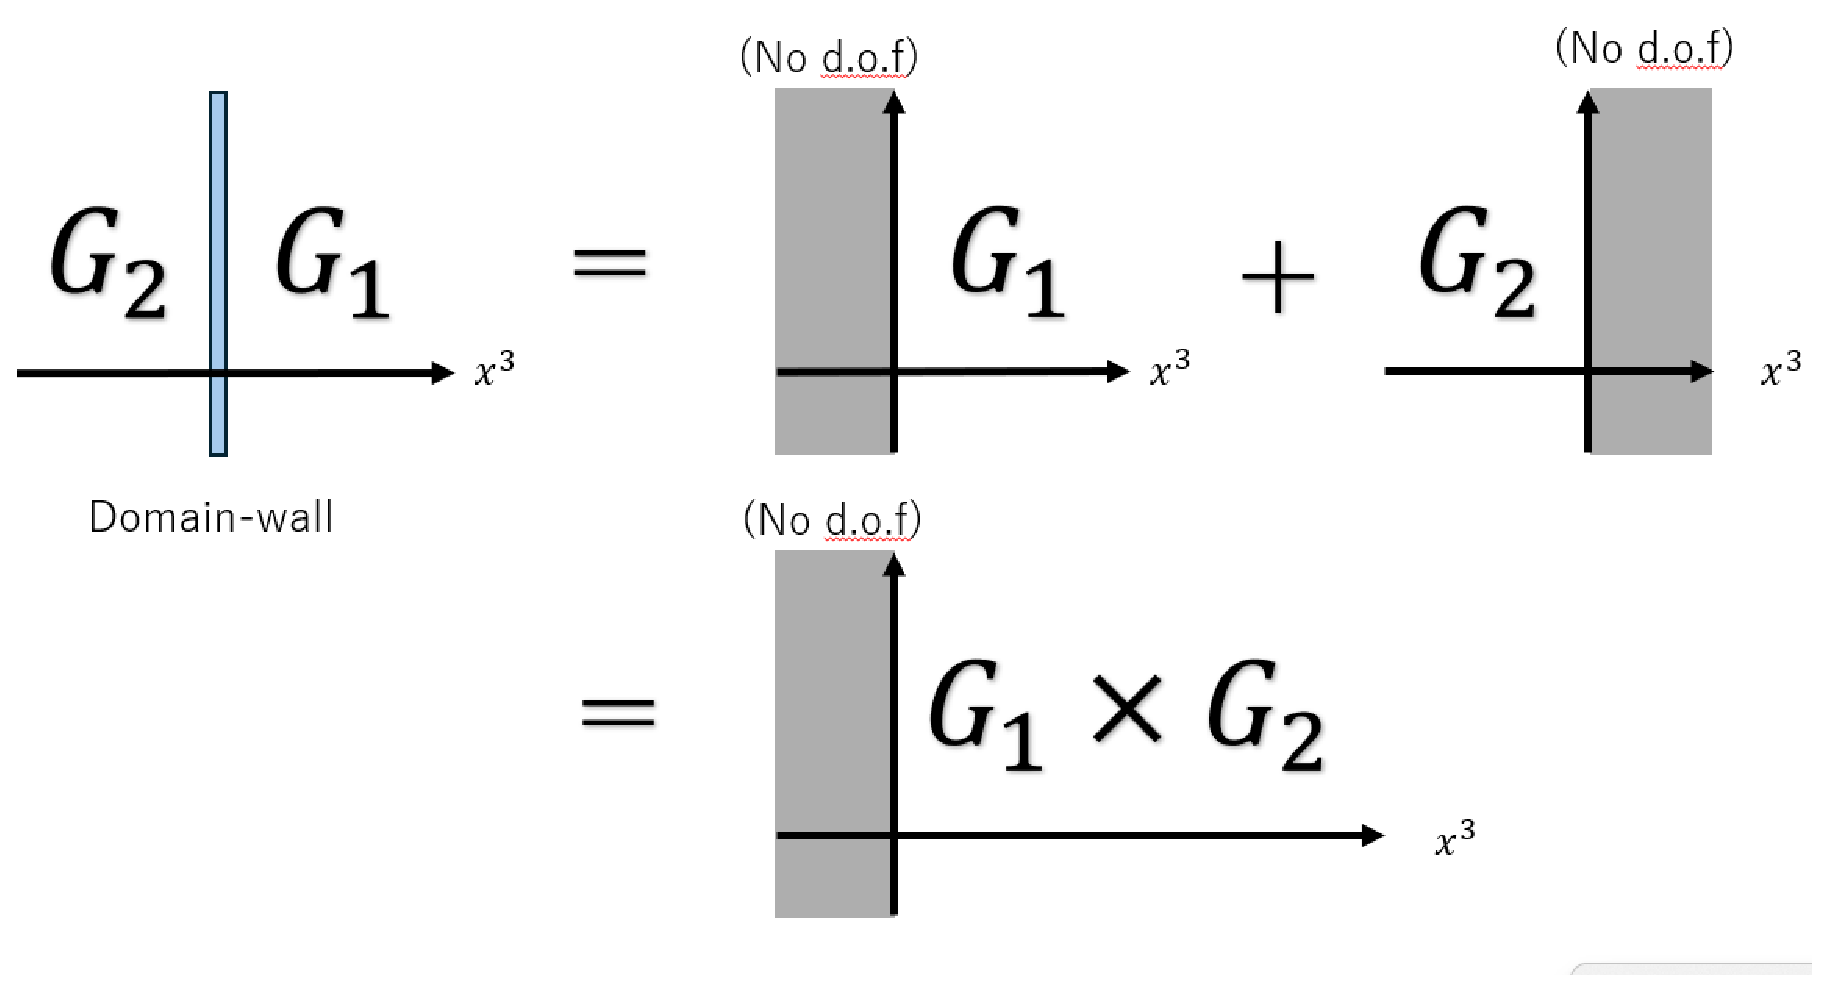
\includegraphics[scale=0.3]{folding.eps}
    \caption{Folding trick}
\end{figure}\\
この図について解説すると、まず、Domain-wallの系は、２つの「適切な」boundary condititonを持つboundary+自由度なしの系に分解できる。\\
\\
次に、ゲージ対称性が$G_{2}$である系に対してParityを作用させたとする。この２つは$x^{3}\geq0$にゲージ対称性を持つ理論となるが、interactionを起こさないため、最終的に$x^{3}\geq 0$上にゲージ対称性$G_{1}\times G_{2}$が存在する系に帰着できる。\\
\\
このように、片方の系を「Folding」することにより、Domain-wall系とBoundary系の等価性を示せる。これが「Folding trick」である。
\end{intuitionbox}
Foldingトリックの帰結として、以下のような双対性を主張できる。
\begin{resultbox}{Domain-wallとBoundary系の双対性}
\begin{align*}
    &\text{(SU(N)ゲージ+su(N+k)ゲージのDomain-wall系)}\\
    \iff &\text{($SU(N)\times su(N+k)$ゲージのBoundary系)}\\
    \text{(parity)}&
\end{align*}    
\end{resultbox}
以下では、Folding-trickを用いた、Domain-wall系とBoundary系の具体的なmappingを考える。Boundary系、Domain-wall系の場は以下のように定義される。
\begin{align*}
    \Phi_{B}=\begin{pmatrix}
        \Phi_{N}(x)\\ \Phi_{N-k}(x)
    \end{pmatrix},\quad 
    \Phi_{D}(x^{3}\geq 0)\in su(N),\quad 
    \Phi_{D}(x^{3}\leq 0)\in su(N+k)
\end{align*}
この時、Folding-trickのマップは以下のように記述される。\\
\begin{resultbox}{Folding-trickのマッピング}
    \begin{enumerate}
    \item Boundary→Domain\\
    この場合、Boundary系の場$\Phi_{B}$を用いて、Domain-wall系の場$\Phi_{D}^{F}$を以下のように定義できる。
    \begin{align*}
        &\Phi_{D}^{F}(x^{3}\geq 0)\equiv \Phi_{B}(x^{3}\geq 0)\\
        &\Phi_{D}^{F}(x^{3}\leq 0)\equiv P\Phi_{B}(-x^{3})P^{-1}
    \end{align*}
    \item Domain→Boundary\\
   この場合、Domain-wall系の場$\Phi_{B}$を用いて、Boundary系の場$\Phi_{D}^{F}$を以下のように定義できる。
    \begin{align*}
        &\Phi_{B}^{F}(x^{3})\equiv \begin{pmatrix}
        \Phi_{D}(x^{3})\\ P\Phi_{D}(-x^{3})P^{-1}
    \end{pmatrix}
    \end{align*}
\end{enumerate}
\end{resultbox}
いずれの場合も、パリティの作用さえ与えれば、場のマッピングも一意に定まる。
\subsubsection{Parityの作用}
この章では、Folding-trickを記述する際に必要となるparityの作用について議論する。\\
\\
ただし、その前に、変換について述べればならない。物理では、主に2種類の変換が存在する。「基底の変換」と、「物理の変換」である。両者の違いは以下の通りである。
\begin{defbox}{物理における変換}
\begin{enumerate}
    \item 基底の変換\\
    基底の変換とは、量そのものは変えない変換である。
    \begin{align*}
        \phi(x)\to \phi'(x')=\phi(x)
    \end{align*}
    \item 物理の変換\\
    物理の変換とは、パラメータの変化に伴い、量そのものを変える変換のことである」。
    \begin{align*}
        \phi(x)\to \phi(x')=U(a)\phi(x)U(a)^{\dagger}
    \end{align*}
\end{enumerate}
\end{defbox}
\begin{intuitionbox}
    \begin{enumerate}
        \item 基底の変換
        基底とは、物理を表すために人類が勝手に用いている基準である。故に、そこを勝手に変更しても物理は変わらないはずである。これを表す変換が、以下の変換である。
        \begin{align*}
        \phi(x)\to \phi'(x')=\phi(x)
    \end{align*}
    ただし、ベクトル場などで基底の変換を考える際は少し注意を伴う。ベクトルの形そのものは変わらないが、それを見るための基底そのものが変化するため、結果として「成分は」変化する。
    \begin{align*}
        &A(x)=A'(x')\\
        \iff&A_{\mu}(x)=\Lambda_{\mu}^{\nu}A'_{\nu}(x')
    \end{align*}
    \item 物理の変換\\
    物理の変換は、例えば「時間発展」が例として挙げられる。例えば場の時間発展は、Heisenberg方程式により記述される。
    \begin{align*}
        &i\frac{d}{dt}\phi(x)=[H,\phi(x)]\\
        \implies&\phi(x')=exp(iHt)\phi(x)exp(-iHt)
    \end{align*}
    これは実際に時間が進むと物理量がどのように変換するか、という実際の「物理の変換」を表している。この例は、定義の変換の一例である。\\
    他の変換として、並進変換などが挙げられる。
    \end{enumerate}
\end{intuitionbox}
以上を踏まえて、Parityを考える際の一般的指針についての議論を行う。ここでいうParity変換とは、Folding-trickへの応用を踏まえて、以下の意味でのParityを考えている。
\begin{defbox}{Parity変換}
    Parityは、実際にxに存在する場を、$x'=-x$に移す、「物理の変換」である。この時、Pをparity変換のオペレータとすると、以下のように記述可能。
    \begin{align*}
        \phi(x)\to \phi(x')=\phi(Px)=P\phi(x)P^{-1}
    \end{align*}
\end{defbox}
この時、パリティ変換の必要条件は、「２回かけて元に戻る」ことである。また、ベクトル場の場合は、同時に軸の向きも変えるため、そのための基底の移り変わりも考慮せねばならない。これらを踏まえると、ベクトル場、スカラー場のParity変換は、以下の通りとなる。
\begin{resultbox}{スカラー場、ベクトル場のParity変換による変化}
    \begin{align*}
        &\phi(x')=P\phi(x)P^{-1}=\pm\phi(x)\\
        &A(x')=PA(x)P^{-1}\iff A_{\mu}(x')=P_{\mu}^{\nu}PA_{\nu}(x)P^{-1} 
    \end{align*}
\end{resultbox}
パリティをかけてーとなる場のことを、「pseudo場」と呼ぶ。Spinor場も、その内積はベクトル場であるため、「pseudoか否かの選択を覗けば」ベクトル場と同様の考え方で変換性を決定できる。\\
\\
問題が、場がPseudoとなるか否かの選択である。これを決めるために、弦理論などでは「変換後にSUSYが不変であるように」pseudoか否かを設定する。\\
ここで言う対称性を保つ変換とは、以下を満たすような変換のことである。(ただし、個人的には定義の動機づけが数学な気がするので、割と受け入れ難い・・・物理的な直感がないものか・・・)
\begin{defbox}{対称性を保つ変換}
    対称性変換を$\delta\phi$,物理の変換を行うオペレータを$P$とする。変換$P$が変換後も対称性を保つとは、以下の関係式を満たすことと定義する\footnote{ただし、アノマリーやセンターなどは考えない。}。
    \begin{align*}
        P(\delta \phi(x))P^{-1}=\delta(P\phi(x)P^{-1})
    \end{align*}
\end{defbox}
ここで、D5-likeなSUSYを保存するようなparityの変換を考えると、pseudoの選択を含めて、parity変換は以下の通りとなる。
\begin{resultbox}{D5-like SUSYを保つparity変換}
    \begin{align*}
        &PX_{a}(x')P^{-1}=-X_{a}(x)\\
        &PY_{m}(x')P^{-1}=Y_{m}(x)\\
        &PA_{\mu}(x')P^{-1}=P_{\mu}^{\nu}A_{\nu}(x)\\
        &P\Psi(x')P^{-1}=B_{1}\Psi(x)
    \end{align*}
\end{resultbox}
\begin{proofbox}
    parityのもとSUSY不変であるという条件は、定義から、以下のような条件式となる。
    \begin{align*}
        &P\delta_{\epsilon} A_{I}(x)P^{-1}=\delta_{\epsilon}(PA_{I}(x)P^{-1})\\
        &P\delta_{\epsilon} \Psi(x) P^{-1}=\delta_{\epsilon}(P\Psi(x) P^{-1})
    \end{align*}
    故に、上記のParity変換式が、これらの等式を満たすことを示せば良い。ここでは、ゲージ場の変換則を満たすことのみを示す。spinor場は同様にやれば良いだけである。
        \begin{align*}
            P(\delta A_{I}(x))P^{-1}&=\bar{\epsilon}\Gamma_{I}(P\Psi(x)P^{-1})\\
            &=\bar{\epsilon}\Gamma_{I}B_{1}\Psi(x')\\
            &=\bar{\epsilon}B_{1}P_{I}^{J}\Gamma_{J}\Psi(x')\\
            &=P_{I}^{J}\bar{\epsilon}\Gamma_{J}\Psi(x')
        \end{align*}
        ただし、上式の変形で、ガンマ行列の交換関係の計算から、以下が成立することを用いた。
        \begin{align*}
            \Gamma_{I}B_{1}=
            \begin{cases}
            -B_{1}\Gamma_{I} \quad(I=3,4,5,6)\\
            B_{1}\Gamma_{I}\quad (I=others)
            \end{cases}
            =P_{I}^{J}B_{1}\Gamma_{J}
        \end{align*}
        ただし、$P_{I}^{J}$は以下で定義される。
        \begin{align*}
            P_{I}^{J}=\begin{cases}
            -\delta_{I}^{J} \quad(I=3,4,5,6)\\
            \delta_{I}^{J}\quad (I=others)
            \end{cases}
        \end{align*}
        一方、スカラー場とベクトル場の変換性を考えると、$PA_{I}(x)P^{-1}=P_{I}^{J}A_{J}(x')$が成立するため、
        \begin{align*}
            \delta_{\epsilon}(PA_{I}(x)P^{-1})&=\delta_{\epsilon}(P_{I}^{J}A_{J}(x'))\\
            &=P_{I}^{J}\bar{\epsilon}\Gamma_{J}\Psi(x')
        \end{align*}
        故に、ゲージ場の変換は確かに保存される。
\end{proofbox}

\subsubsection{ゲージ群の直和構造とaction}
上記の章では、Domain-wall系が、リー代数の直和をゲージ対称性にもつ、Boundary系のSYMと等価であることを見た。これのダイナミクスを決定するため、この章では直和ゲージ群のゲージ理論のアクションを眺める。\\
\\
ゲージ群$g=g_{1}+g_{2}\cdots $の一般的なアクションは以下の通りである。注目すべきは、ゲージ群が直和の場合、それぞれでの構造定数が独立であることが許される点である。
\begin{align*}
    S=-\frac{1}{4}\int d^{d}x \frac{1}{e_{1}^{2}}F_{a}^{\mu\nu}F^{a}_{\mu\nu}+\frac{1}{e_{2}^{2}}G_{\mu\nu}^{m}G^{\mu\nu}_{m}+\cdots
\end{align*}
ここで、添字(a,m)は、ゲージ群$g_{1},g_{2}$の添字である。\\
matter-contentsを加えたアクションを考えても、リー代数の表現のトレースを用いて、以下のように記述できる。
\begin{align*}
    S=\frac{1}{2}\int d^{d}x \frac{1}{e_{1}^{2}}Tr_{g_{1}}(\cdots)+\frac{1}{e_{2}^{2}}Tr_{g_{2}}(\cdots)+\cdots
\end{align*}
この時、注意すべきはカレントの構造である。ゲージ群が$g_{1},g_{2}$単体の時に、アクションがカレントを持っていたとする。今の場合、1/2-BPS分のSUSYを保つカレントである。
この時、アクションの変分は以下のように記述できる。
\begin{align*}
    S
    =\int d^{d}x (\partial_{\mu}\epsilon)(\frac{1}{e_{1}^{2}}j_{1}^{\mu}+\frac{1}{e_{2}^{2}}j_{2}^{\mu}+\cdots)
\end{align*}
故に、ゲージ群が直和の時のカレントの保存則は、「各々のカレントが保存するのではなく、全体で差し引きゼロであれば良い」ことを意味する\footnote{各々が
0であるという条件は、十分条件であって必要条件ではない}。式的には以下である。
\begin{align*}
    \partial_{\mu}J^{\mu}=\partial_{\mu}(\frac{1}{e_{1}^{2}}j_{1}^{\mu}+\frac{1}{e_{2}^{2}}j_{2}^{\mu}+\cdots)
\end{align*}
故に、今まで考えていた保存条件とはまた異なるため、1/2-BPS境界条件を求める手続きを再考しなければならない。\\
\\
では、どこまで戻るべきなのだろうか？それを考えるため、境界条件を考えるために使用した流れを抽象化してチャート化する。
\begin{setupbox}{ゲージ群の1/2-BPS境界条件の導出法}
\begin{enumerate}
    \item カレントを求める
    \begin{align*}
        Tr(\bar{\epsilon}\Gamma^{IJ}F_{IJ}\Gamma^{3}\Psi)|_{x^{3}=0}=0
    \end{align*}
    \item (カレント)=0という式をローレンツ変換性から分解
    \begin{align*}      
        \begin{cases}
             0&=\bar{\epsilon}_{0}(F_{\mu\nu}-\epsilon_{\mu\nu\lambda}F^{3\lambda}B_{0})\theta_{0}\\
    0&=(D_{\mu}X_{a})(\bar{\epsilon}B_{2}\theta_{0})\\
    0&=(D_{\mu}Y_{m})(\bar{\epsilon}B_{1}\theta_{0})\\
    0&=[X_{m},Y_{a}](\bar{\epsilon}B_{0}\theta_{0})\\
    0&=\bar{\epsilon}_{0}([X_{b},X_{c}]-\epsilon_{abc}D_{3}X_{a}B_{1})\theta_{0}\\
    0&=\bar{\epsilon}_{0}([Y_{m},Y_{n}]-\epsilon_{mnl}D_{3}Y_{l}B_{2})\theta_{0}
        \end{cases}
    \end{align*}
    \item 分解した各項を、ゲージ群の内積の直交構造でさらに分解
    \begin{align*}
        &\begin{cases}
            \bar{\epsilon}_{0}(F^{h}_{\mu\nu}-\epsilon_{\mu\nu\lambda}F_{3\lambda}^{h}B_{0})\theta_{0}^{h}=0,\quad
    \bar{\epsilon}_{0}(F^{\perp}_{\mu\nu}-\epsilon_{\mu\nu\lambda}F_{3\lambda}^{\perp}B_{0})\theta_{0}^{\perp}=0\\
    (D_{\mu}X_{a}^{h})(\bar{\epsilon}B_{2}\theta_{0}^{h})=0,\quad
    (D_{\mu}X_{a}^{\perp})(\bar{\epsilon}B_{2}\theta_{0}^{\perp})=0\\
    (D_{\mu}Y_{m}^{h})(\bar{\epsilon}B_{1}\theta_{0}^{h})=0,\quad
    (D_{\mu}Y_{m}^{\perp})(\bar{\epsilon}B_{1}\theta_{0}^{\perp})=0\\
    [X_{m},Y_{a}]^{h}(\bar{\epsilon}B_{0}\theta_{0}^{h})=0,
    \quad[X_{m},Y_{a}]^{\perp}(\bar{\epsilon}B_{0}\theta_{0}^{\perp})=0\\
    \bar{\epsilon}_{0}([X_{b},X_{c}]^{h}-\epsilon_{abc}D_{3}X_{a}^{h}B_{1})\theta_{0}^{h}=0\\
    \bar{\epsilon}_{0}([X_{b},X_{c}]^{\perp}-\epsilon_{abc}D_{3}X_{a}^{\perp}B_{1})\theta_{0}^{\perp}=0\\
    \bar{\epsilon}_{0}([Y_{m},Y_{n}]^{h}-\epsilon_{mnl}D_{3}Y^{h}_{l}B_{2})\theta_{0}^{h}=0\\
    \bar{\epsilon}_{0}([Y_{m},Y_{n}]^{\perp}-\epsilon_{mnl}D_{3}Y^{\perp}_{l}B_{2})\theta_{0}^{\perp}=0
        \end{cases}
    \end{align*}
    (ここまで一般的な手続き)
    \item それっぽそうな解を代入して条件を満たす境界条件を検証
    \begin{equation}
\begin{split}
     F_{3\mu}^{h}|&=0,\quad
    F_{\mu\nu}^{\perp}|=0\\
    \vec{X}^{h}|&=0,\quad
    (\varepsilon_{abc}D_{3}\vec{X}_{a}^{\perp}-[X_{b}^{\perp},X_{c}^{\perp}]^{\perp})|=0\\
    \vec{Y}^{\perp}|&=0,\quad
    D_{3}\vec{Y}^{h}|=0\\
    B_{1}\Psi^{h}|&=\Psi,\quad B_{1}\Psi^{\perp}=-\Psi^{\perp}
\end{split}
\end{equation}
\end{enumerate}
\end{setupbox}
この手続きは、直和リー代数$g_{1}\oplus g_{2}$の表現$(X_{1},X_{2}),(Y_{1},Y_{2})$の内積を、以下のように定義すると、直和リー群のSYMでもトレース可能である。
\begin{defbox}{直和リー代数の内積}
    \begin{align*}
    <(X_{1},X_{2}),(Y_{1},Y_{2})>\equiv \frac{1}{e_{1}^{2}}Tr_{g_{1}}(X_{1}Y_{1})+\frac{1}{e_{2}^{2}}Tr_{g_{2}}(X_{2}Y_{2})
\end{align*}
\end{defbox}
この時に決定的にゲージ群が１つの場合と異なるのは、直交補空間$h^{\perp}$の構造である。直交補空間は、内積によって変化するためである。このことを念頭に入れ、Domain-wall解の境界条件を決定する。

\subsubsection{Domain-wall condition}
今までの議論により、Domain-wall系の境界条件(Dommain-wall condition)を考えるための道具立ては全て揃った。とはいえ、全てのDomai-wallを考えるのは、Boundary上で許される部分群を全て考えねばならないため、非常に面倒臭い。\\
それゆえ、実用上重要となる、以下の場合のDomain-wallへのmappingに解析を留める。
\begin{enumerate}
    \item h=0の場合
    \item hがdiagonalの場合
\end{enumerate}
これらの場合のDomain-wall系のmappingを考える。これを行うために、先ほどのParityの議論に従い、Folding-trickした場合の場のマッピングを考える。
\begin{defbox}{SYMのDomain-wall系へのマッピング}
    Folding-trickを用いると、Domain-wall系の場は以下のように記述される。
    \begin{align*}
        &\begin{cases}
           X_{D}^{a}(x^{3}\geq 0)\equiv X^{a}_{N}(x^{3})\\
           X_{D}^{a}(x^{3}\leq 0)\equiv -X^{a}_{M}(-x^{3})
        \end{cases}\\
        \\
        &\begin{cases}
           Y_{D}^{m}(x^{3}\geq 0)\equiv Y^{m}_{N}(x^{3})\\
           Y_{D}^{m}(x^{3}\leq 0)\equiv Y^{m}_{M}(-x^{3})
        \end{cases}\\
        \\
        &\begin{cases}
           A_{D}^{\mu}(x^{3}\geq 0)\equiv A^{\mu}_{N}(x^{3})\\
           A_{D}^{\mu}(x^{3}\leq 0)\equiv P^{\mu}_{\nu}A^{\nu}_{M}(-x^{3})
        \end{cases}\\
        \\
        &\begin{cases}
           \Psi_{D}(x^{3}\geq 0)\equiv \Psi_{N}(x^{3})\\
           \Psi_{D}(x^{3}\leq 0)\equiv B_{1}\Psi_{M}(-x^{3})
        \end{cases}
    \end{align*}
\end{defbox}
\begin{enumerate}
    \item h=0の場合\\
    この場合、$h^{\perp}=su(N)\oplus su(N+k)$であるため、Boundary-conditionは以下の通りである。
    \begin{equation}
\begin{split}
    F_{\mu\nu}|&=0\\
    D_{3}\vec{X}|&=0\\
    \vec{Y}|&=0\\
    B_{1}\Psi&=\Psi
\end{split}
\end{equation}
先ほど議論したmappingに従い、Domain-wall上の境界条件を求めると、以下の通りになる。
\begin{resultbox}{h=0に対応するDomain-wall上の(b.c.)}
    \begin{align*}
    &Y_{D}(x^{3}\to +0)=Y_{D}(x^{3}\to -0)=0\\
    &A^{\mu}_{D}(x^{3}\to +0)=A^{\mu}_{D}(x^{3}\to -0)=0\\
    &D_{3}X_{D}(x^{3}\to +0)=D_{3}X_{D}(x^{3}\to -0)=0
\end{align*}
この場合は、「左側と右側で、独立にD5-likeかつBoundary上のゲージ群が自明であるような境界条件を与える」という描像に対応する。
\end{resultbox}

\item hが「diagonal部分群」の場合\\
まずhがdiagonalであるとは、以下を満たすことである。
\begin{resultbox}{diagonal部分群}
    $g=su(N)\oplus su(N+k)$とする。この時、isometry(等長写像)、つまり以下を満たす写像を定義する。
    \begin{align*}
        i:su(N)\to su(N+k),\quad 
    i(X)\equiv\begin{pmatrix}
        X & 0\\ 0 & 0
    \end{pmatrix}
    \end{align*}
    この時、部分群として、以下のようなものが自然に存在する。
    \begin{align*}
        &h=\{(X,i(X))\,|\,X\in su(N)\}
    \end{align*}
    この部分群hのことを、「diagonal部分群」と呼ぶ。
\end{resultbox}
この時、gのうち、hの直交補空間は以下の通りである。
\begin{resultbox}{hの直交補空間}
    \begin{align*}
        h^{\perp}=\{(X,-\frac{e_{2}^{2}}{e_{1}^{2}}i(X)+A)\,|\,A\in su(N+k),<A,i(M)>=0 \}
    \end{align*}
ただし、Mはsu(N)上の任意の元である。
\end{resultbox}
\begin{proofbox}
    まず、以下のような性質が成立する。証明は自明なので行わない。
    \begin{resultbox}{embeddingの内積}
        \begin{align*}
        tr_{N}(XY)=tr_{N+k}(i(X)i(Y))
    \end{align*}
    \end{resultbox}
    この時、h上の場を$(X,i(X))$とする。次に、g上の任意の元を、以下のように取る。
    \begin{align*}
        (Z,Y)=(Z,-i(Z)+\{i(Z)+Y\})=(Z,-i(Z)+A)
    \end{align*}
先ほどの定義に従うと、ゲージ群$su(N)\oplus su(N+k)$の内積は以下のように記述される。
\begin{align*}
    <(X_{1},X_{2}),(Y_{1},Y_{2})>\equiv \frac{1}{e_{1}^{2}}Tr_{N}(X_{1}Y_{1})+\frac{1}{e_{2}^{2}}Tr_{N+k}(X_{2}Y_{2})
\end{align*}
この時、gの元とhの元の内積は以下の通りである。
\begin{align*}
    &<(X,i(X)),(Z,-i(Z)+A)>_{N\oplus (N+k)}\\
    &=tr_{N}(XZ)-tr_{N+k}(i(X)i(Z))+tr_{N+k}(i(X),A)\\
    &=tr_{N+k}(i(X)A)
\end{align*}
g上の元が直交補空間上にいると思うと、上記の内積が０となければならない。\\
故に、直交補空間である必要十分条件は、$<A,i(X)>=0$である。
\end{proofbox}
また後々、Foldingした結果、どこがどこに映るかをわかりやすくするため、以下のようなnotationを採用して議論を進める。
\begin{defbox}{リー代数のnotation}
    \begin{align*}
        \begin{pmatrix}
           su(N) \\ U \\ U^{\perp}
        \end{pmatrix}
    \end{align*}
    この時、Uはembeddingによるsu(N+k)内のsu(N)部分空間、$U^{\perp}$はUの直交補空間である。
    \begin{align*}
        &U=\{i(X)\in su(N+k)\,|\,X\in su(N)\}\\
        &U^{\perp}=\{X\in su(N+k)\,|\,\forall Y\in su(N),<X,i(Y)>=0 \}
    \end{align*}
\end{defbox}
このnotationの下、Folding-trickは、第2,第3成分をParityして右側へ持っていく操作である。\\
\\
以上のセットアップを元に、hを部分群としたBoundary系をFoldingした後の、Domain-wall上の境界条件を考える。まず、Boundary系での$h,h^{\perp}$上での場は以下の通りである。
\begin{resultbox}{Boundary系での場}
    \begin{align*}
    &\Phi^{h}(x)=\begin{pmatrix}
        \phi_{N}(x)\\ \phi_{N}(x) \\ 0
    \end{pmatrix}\\
    &\Phi^{\perp}(x)=\begin{pmatrix}
        \phi_{N}(x)\\ -\frac{e^{2}_{2}}{e^{2}_{1}}\phi_{N}(x) \\ \phi_{k}(x)
    \end{pmatrix}
\end{align*}
\end{resultbox}
このため、Boundary上の境界条件は、以下のようになる。ただし、見やすいように、ゲージ固定は$A=0$を採用した。
\begin{resultbox}{diagonal部分群の時のD5-like境界条件}
    \begin{align*}
        &X^{h}|=0 \implies X|=\begin{pmatrix}
        X_{N}\\ -\frac{e^{2}_{2}}{e^{2}_{1}}X_{N} \\ X_{\perp}
    \end{pmatrix}\\
    & Y^{\perp}|=0 \implies Y|=\begin{pmatrix}
        Y_{N}\\ Y_{N} \\0
    \end{pmatrix}\\
    & A^{\perp}|=0 \implies A|=\begin{pmatrix}
        A_{N}\\ A_{N} \\0
    \end{pmatrix}\\
    &\Psi|=\begin{pmatrix}
        \Psi^{+}_{N}+\Psi^{-}_{N}\\ \Psi^{+}_{N}-\frac{e_{1}^{2}}{e_{2}^{2}}\Psi^{-}_{N} \\\Psi_{\perp}^{-}
    \end{pmatrix}
    \end{align*}
\end{resultbox}
ただし、spinorの$\pm$の添え字は$B_{1}$の固有値を表す。\\
\\
この時、各パリティのマップを用いて、場を射影することができる。この場合、Domain-wall上の場は以下のようになる。
\begin{resultbox}{Domain-wall系で境界付近での場の振る舞い}
    \begin{align*}
        \begin{cases}
            X_{D}(x^{3}=+ 0)&=X_{N}(x^{3})\\
            Y_{D}(x^{3}=+0)&=Y_{N}(x^{3})\\
            A^{\mu}_{D}(x^{3}=+ 0)&=A^{\mu}_{N}(x^{3})\\
            \Psi_{D}(x^{3}=+ 0)&=\Psi_{N}(x^{3})\\
        \end{cases}\\
        \\
        \begin{cases}
            X_{D}(x^{3}=- 0)&=
            \begin{pmatrix}
                \frac{e^{2}_{2}}{e^{2}_{1}}X_{N}(-x^{3})\\
                -X_{k}(-x^{3})
            \end{pmatrix}\\
            Y_{D}(x^{3}=- 0)&=\begin{pmatrix}
                Y_{N}(-x^{3})\\
                Y_{k}(-x^{3})
            \end{pmatrix}\\
            A^{\mu}_{D}(x^{3}=- 0)&=\begin{pmatrix}
                A^{\mu}_{N}(-x^{3})\\
                A^{\mu}_{k}(-x^{3})
            \end{pmatrix}\\
            \Psi_{D}(x^{3}=- 0)&=\begin{pmatrix}
                \Psi^{+}_{N}+\frac{e_{1}^{2}}{e_{2}^{2}}\Psi^{-}_{N} \\-\Psi_{\perp}^{-}
            \end{pmatrix}
        \end{cases}
    \end{align*}
\end{resultbox}
このマップから、特にN成分に関する境界条件は以下のように記述される。
\begin{align*}
    (X_{D}(x^{3}=-0))_{N}&=\frac{e_{2}^{2}}{e_{1}^{2}}X_{D}(x^{3}=+0)\\
    (Y_{D}(x^{3}=-0))_{N}&=Y_{D}(x^{3}=+0)\\
    (A^{\mu}_{D}(x^{3}=-0))_{N}&=A^{\mu}_{D}(x^{3}=+0)\\
    \Psi^{+}_{N}+\frac{e_{1}^{2}}{e_{2}^{2}}\Psi^{-}_{N}|_{x^{3}=-0}&=\Psi_{N}(x^{3})
\end{align*}
特に、$e_{1}=e_{2}$の時Domain-wall境界条件を述べることは重要である。上記の射影後の式に$e_{1}=e_{2}$を代入すると、以下のような境界条件となることが自然に示せる。
\begin{resultbox}{カップリングが等しい場合のDomain-wall上の境界条件}
    まず、su(N+k)内に以下のような部分群が自然に存在。
    \begin{gather*}
        h=\{i(X)\in su(N+k)\,|\,X\in su(N)\}\\
        su(N+k)=h\oplus h^{\perp}
    \end{gather*}
    この場合、場は以下のように分解される。
    \begin{gather*}
        \Phi=\Phi^{h}+\Phi^{\perp}\\
        (\Phi^{h}\in h,\quad \Phi^{\perp}\in h^{})
    \end{gather*}
    そしてD5-like SUSYを保つDomain-wall上の境界条件は、以下のようになる。
    \begin{enumerate}
        \item $h$成分の境界条件
        \begin{align*}
            \Phi^{h}(x^{3}=+0)=\Phi(x^{3}=-0)
        \end{align*}
        \item 直交補空間上の境界条件
        \begin{gather*}
            (\varepsilon_{abc}D_{3}\vec{X}_{a}^{\perp}-[X_{b}^{\perp},X_{c}^{\perp}]^{\perp})|_{x^{3}=+0,x^{2}\geq 0}=0\\
            \vec{Y}^{\perp}|_{x^{3}=+0,x^{2}\geq 0}=0\\
            B_{1}\Psi^{\perp}|_{x^{3}=+0,x^{2}\geq 0}=\Psi^{\perp}
        \end{gather*}
    \end{enumerate}   
\end{resultbox}
\end{enumerate}
以上より、応用上重要な場合のDomain-wall上の境界条件を導出できた。当然、量子論の場合は上記の境界条件がオペレータの関係式となる。


\subsubsection{Domain-wall系のモジュライ空間}
前節で境界条件を入手できたので、それのVEVを考えることもできる。ただし、Bulk上の制約は変わらず、境界条件のみ非自明な変更点が出現する。ここでは、特に非自明な結果となる、「diagonal部分群から得られたDomain-wall」に関してのモジュライ空間を構成する。なお、簡単のため、Y=0とする。\\
\\
X場に関しての境界条件は、以下のように記述可能である。
\begin{resultbox}{X場の境界条件}
    \begin{align*}
        &(X_{D}(x^{3}=-0))_{N}=\frac{e_{2}^{2}}{e_{1}^{2}}X_{D}(x^{3}=+0)\\
        &D_{3}X_{D}^{k}-[X_{D}^{k},X_{D}^{k}]^{k}|_{x^{3}=-0}=0
    \end{align*}
\end{resultbox}
これはオペレータ同士の関係式であるため、当然、VEVもこの関係式を持つ必要がある。故に、特にX場のVEVが満たすべき関係式は以下の通りである。以降この小節では、VEVを表す括弧は省略するが、少なくともこの小節内では、括弧は常に、暗につけていることに注意が必要である。
\begin{resultbox}{Domain-wallのX場のVEV-constraint}
    \begin{align*}
        &\bar{\epsilon}_{0}([X_{D}^{b},X_{D}^{c}]-\epsilon_{abc}D_{3}X_{D}^{a})=0\\
        &(X_{D}(x^{3}=-0))_{N}=\frac{e_{2}^{2}}{e_{1}^{2}}X_{D}(x^{3}=+0)\\
        &D_{3}X_{D}^{k}-[X_{D}^{k},X_{D}^{k}]^{k}|_{x^{3}=-0}=0
    \end{align*}
\end{resultbox}
以下、これを満たす解を構築する。
\begin{enumerate}
    \item 定数型の解\\
    上記を満たす解として、例えば定数型の解を上げる。この際、bulkの方程式から、定数型の解は、以下のような形になる。
    \begin{align*}
    [X_{b},X_{c}]=0\iff 
    \begin{cases}
    &X_{a}(x^{3}\geq0)=\begin{pmatrix}
a_1 & 0 & \cdots & 0 \\
0 & a_2 & \cdots & 0 \\
\vdots & \vdots & \ddots & \vdots \\
0 & 0 & \cdots & a_n
\end{pmatrix}\\  
\\
&X_{a}(x^{3}\leq0)=\begin{pmatrix}
a_1' & 0 & \cdots & 0 \\
0 & a_2' & \cdots & 0 \\
\vdots & \vdots & \ddots & \vdots \\
0 & 0 & \cdots & a_{n+k}'
\end{pmatrix}
    \end{cases}
\end{align*}
この時、境界条件から、以下のような条件が出現する。
\begin{align*}
    a'_{i}=\frac{e_{2}^{2}}{e_{1}^{2}}a_{i}
\end{align*}
他に条件付けはなされない。この縛りのもと、固有値が異なるVEVを集めたものが、モジュライ空間に相当する。
    \item Pole型の解\\
    以下、Pole解型のModuli空間を考える。ここでいうPole解とは以下である。
    \begin{align*}
    \begin{cases}
         X_{D}^{a}(x^{3}\geq 0)=-\frac{t^{a}}{x^{3}}\\
         X_{D}^{a}(x^{3}\leq 0)=-\frac{t'^{a}}{x^{3}}
    \end{cases}
    \end{align*}
    まずは、Bulk上のEOMから、
    \begin{align*}
        [t^{b},t^{c}]=\varepsilon_{abc}t^{a}
    \end{align*}
    この時、境界条件の連続性の部分から、
    \begin{align*}
        t^{a}=0,\quad t'^{a}\in \begin{pmatrix}
            0 \\
            V_{k}
        \end{pmatrix}
    \end{align*}
    これを満たす場合、他の境界条件からのconstraintは存在しない。\\
    \\
    故に、この場合のモジュライ空間は、以下の写像の分類の結果に等しい。
    \begin{align*}
        \rho:su(2)\to su(k)
    \end{align*}
    この写像の分類はすでに完了している。故に、Pole解型のモジュライ空間は以下のように記述される。
    \begin{resultbox}{Domain-wallのPole解のモジュライ空間}
        \begin{align*}
        k=\sum_{i}k_{i}
    \end{align*}
    \end{resultbox}
\end{enumerate}

\section{CrossしたBrane系}
以下では、研究内容である、Domain-wallがクロスしたような場合について考える。ここでは一般的なBraneの配位ではなく、両方D5であるような、特別な配位の低エネルギーに相当するようなゲージ理論の境界条件を考えていく。
\subsection{Braneの配位とSUSYの保存}
まずは考えるBraneの配位について述べる。今章では、以下の図のような配位を考える。\\
この配位の時の、SUSYの保ち方は以下の通りとなる。
\begin{align*}
    \bar{\varepsilon}B_{1}=\bar{\varepsilon},&\quad \bar{\varepsilon}C_{2}=\bar{\varepsilon}\\
    B_{1}&=\Gamma^{3456}\\
    C_{2}&=\Gamma^{2789}
\end{align*}
\begin{resultbox}{SUSYを保つ量}
    この系で保つSUSYは$\frac{1}{4}$-BPS分である。
\end{resultbox}
\begin{proofbox}
    Projectionを構成して、そこの固有値が1となる部分の次元を数える。projectionの固有値は1,0であるため、トレースの値がそのまま固有空間の次元となる。\\
    特に今の場合、双方のProjection同士は可換であるため、同時対角化可能で、両方の固有値が1となる領域も同様の方法で調べられる。
    \begin{align*}
        \Pi_{B}=tr(\frac{I+B_{1}}{2}),\quad \Pi_{C}=tr(\frac{I+C_{2}}{2})
    \end{align*}
    この時、両方の固有値が1の固有部分空間の次元は、先ほど述べた通り以下で計算される。
    \begin{align*}
        tr(\Pi_{B}\Pi_{C})&=\frac{1}{4}Tr(I+B_{1}+C_{2}+B_{1}C_{2})\\
        &=\frac{1}{4}Tr(I)=4
    \end{align*}
    ただし、途中でトレースの巡回性から成り立つ式である、$trB_{1}=trC_{2}=trB_{1}C_{2}=0$を用いた。
    故に、固有空間が$16\to4$へ減少するため、保つSUSYは1/4-BPSである。
\end{proofbox}
\subsection{Cross-Boundary系($x^{2},x^{3}\geq 0$)}
以下では、ひとまずBoundary系について考察する。ここでいうBoundary系とは、下図のように、$x^{2},x^{3}=0$上にBoundaryが配置されている系のことを指す。
\subsubsection{境界条件}
まず、この系における1/4-BPS分のSUSYを保つような境界条件を考える。境界条件を考える際の指針は単一境界の場合と同じで、「カレントの流出入がBoundary上で0となる」ことである。このため、境界条件は以下の式により導出される。
\begin{defbox}{２つBoundaryのある1/4-BPS境界条件}
    2つ境界のある系でで1/4-BPS分のSUSYを保つことは、以下の式を場$(X,Y,A,\Psi)$が満たすことに等しい。
    \begin{align*}
        Tr(\bar{\epsilon}\Gamma^{IJ}F_{IJ}\Gamma^{3}\Psi)|_{x^{3}=0}=0\\
        Tr(\bar{\epsilon}\Gamma^{IJ}F_{IJ}\Gamma^{2}\Psi)|_{x^{2}=0}=0
    \end{align*}
\end{defbox}
以下では、これを満たすような境界条件を考察する。セットアップは、何度も再掲するが、以下の通りであろう。\\
\begin{setupbox}{ゲージ群の1/2-BPS境界条件の導出法}
\begin{enumerate}
    \item カレントを求める
    \item (カレント)=0という式をローレンツ変換性から分解
    \item 分解した各項を、ゲージ群の内積の直交構造でさらに分解
    (ここまで一般的な手続き)
    \item それっぽそうな解を代入して条件を満たす境界条件を検証
\end{enumerate}
\end{setupbox}
ただし、今の場合、2つ目の式からやり直さなければならない。単一のBoundaryの議論では、ローレンツ変換性によって境界条件が満たすべき式をいくつかに分解したが、Boundaryが２つ存在する場合は、まずそのローレンツ変換性が異なるためである。\\
\\
しかし、境界条件は本来ローカルなものである。相対論的な場の理論では、同時刻のローカルなものは互いに影響を及ぼさないはずである。故に、互いの境界条件については、もう片方の境界条件が存在しないものだと思って計算しても問題ないはずである\footnote{ただし、実際本当に問題ないかは非自明なので、構成したものが本当に解になるかは、全部代入して確かめなければならない}。以下では、そのような状況の特解を探す。\\
\\
$x^{3}=0$上の解は既に求めたように、以下の通りである。ただし、この時のhは$x^{3}=0$上のゲージ群である。
\begin{resultbox}{$x^{3}=0$の境界条件}
        \begin{equation}
\begin{split}
     F_{3\mu}^{h}|&=0,\quad
    F_{\mu\nu}^{\perp}|=0\\
    \vec{X}^{h}|&=0,\quad
    (\varepsilon_{abc}D_{3}\vec{X}_{a}^{\perp}-[X_{b}^{\perp},X_{c}^{\perp}]^{\perp})|=0\\
    \vec{Y}^{\perp}|&=0,\quad
    D_{3}\vec{Y}^{h}|=0\\
    B_{1}\Psi^{h}|&=\Psi,\quad B_{1}\Psi^{\perp}=-\Psi^{\perp}
\end{split}
\end{equation}
\end{resultbox}
一方、$x^{2}=0$の方の境界条件は、一番一般的には以下のように記述される。ただし、この時のhは$x^{2}=0$上のゲージ群である。
\begin{resultbox}{$x^{2}=0$の境界条件}
\begin{align*}
&F^{h}_{2\lambda}=0,\quad F^{\perp}_{\mu\nu}=0\\
&D_{2}X^{h}=0,\quad X^{\perp}=0\\
&Y^{h}=0,\quad \varepsilon_{lmn}D_{2}Y_{l}^{\perp}-[Y_{m}^{\perp},Y_{n}^{\perp}]^{\perp}=0\\
&C_{2}\Psi^{h}=\Psi^{h},\quad C_{2}\Psi^{\perp}=-\Psi^{\perp}
\end{align*}
\end{resultbox}
\begin{proofbox}
方針は上述したセットアップの通りである。\\
まず、演算子として以下を定義する。
\begin{align*}
    C_{0}\equiv B_{0},\quad C_{1}\equiv \Gamma^{2456},\quad C_{2}\equiv \Gamma^{3789}
\end{align*}
この時、ガンマ行列の積を、以下のような組に分解する。ただし、$x^{3}=0$の時と異なり、$\mu,\nu=0,1,3$であることに注意せねばならない。
\begin{equation}\begin{split}
    \text{(1)}&=\{\Gamma^{\mu\nu},\Gamma^{ab},\Gamma^{mn}\}\\
    \text{(2)}&=\{\Gamma^{\mu2},\Gamma^{2a},\Gamma^{2m}\}\\
    \text{(3)}&=\{\Gamma^{\mu a},\Gamma^{\mu m},\Gamma^{am}\}
\end{split} \end{equation}
この時、(1)は$SO(1,2)\times SO(3)\times SO(3)$の生成子である。(2),(3)は、以下のように分解できる。
\begin{equation}\begin{split}
    \Gamma^{2\lambda}&=-\frac{1}{2}\epsilon^{\lambda}_{\mu\nu}\Gamma^{\mu\nu}C_{0}\bar{\Gamma}\\
    \Gamma^{2c}&=-\frac{1}{2}\epsilon^{c}_{ab}\Gamma^{ab}C_{1}\\
     \Gamma^{2l}&=-\frac{1}{2}\epsilon^{l}_{mn}\Gamma^{mn}C_{2}
\end{split} \end{equation}
\begin{equation}\begin{split}
    \Gamma^{\mu a}&=-\frac{1}{4}\epsilon^{\mu\nu\lambda}\epsilon^{abc}\Gamma_{\nu\lambda}\Gamma_{bc}C_{2}\bar{\Gamma}\\
    \Gamma^{\mu l}&=-\frac{1}{4}\epsilon^{\mu\nu\lambda}\epsilon^{lmn}\Gamma_{\nu\lambda}\Gamma_{mn}C_{1}\bar{\Gamma}\\
    \Gamma^{al}&=-\frac{1}{4}\epsilon^{abc}\epsilon^{lmn}\Gamma_{bc}\Gamma_{mn}C_{0}
\end{split} \end{equation}
故に、明らかに(1),(2)は同じ空間を貼り、(1),(3)は線型独立である。\\
\\
このため、境界条件の式は、以下のように分解可能である。ただし、各項のFの値はすでにX,Y,Aを用いて書き換えている。
\begin{equation}\label{true_b.c.}
\begin{split}
     0&=\bar{\epsilon}_{0}(F_{\mu\nu}-\epsilon_{\mu\nu\lambda}F^{2\lambda}C_{0})\theta_{0}\\
    0&=(D_{\mu}X_{a})(\bar{\epsilon}C_{2}\theta_{0})\\
    0&=(D_{\mu}Y_{m})(\bar{\epsilon}C_{1}\theta_{0})\\
    0&=[X_{m},Y_{a}](\bar{\epsilon}C_{0}\theta_{0})\\
    0&=\bar{\epsilon}_{0}([X_{b},X_{c}]-\epsilon_{abc}D_{2}X_{a}C_{1})\theta_{0}\\
    0&=\bar{\epsilon}_{0}([Y_{m},Y_{n}]-\epsilon_{mnl}D_{2}Y_{l}C_{2})\theta_{0}
\end{split}
\end{equation}
さらに、ゲージ群を$g=h\oplus h^{\perp}$と分解することにより、上記の式は以下の通り分解できる。
\begin{align*}
    \begin{cases}
            \bar{\epsilon}_{0}(F^{h}_{\mu\nu}-\epsilon_{\mu\nu\lambda}F_{2\lambda}^{h}C_{0})\theta_{0}^{h}=0,\quad
    \bar{\epsilon}_{0}(F^{\perp}_{\mu\nu}-\epsilon_{\mu\nu\lambda}F_{2\lambda}^{\perp}C_{0})\theta_{0}^{\perp}=0\\
    (D_{\mu}X_{a}^{h})(\bar{\epsilon}C_{2}\theta_{0}^{h})=0,\quad
    (D_{\mu}X_{a}^{\perp})(\bar{\epsilon}C_{2}\theta_{0}^{\perp})=0\\
    (D_{\mu}Y_{m}^{h})(\bar{\epsilon}C_{1}\theta_{0}^{h})=0,\quad
    (D_{\mu}Y_{m}^{\perp})(\bar{\epsilon}C_{1}\theta_{0}^{\perp})=0\\
    [X_{m},Y_{a}]^{h}(\bar{\epsilon}C_{0}\theta_{0}^{h})=0,
    \quad[X_{m},Y_{a}]^{\perp}(\bar{\epsilon}C_{0}\theta_{0}^{\perp})=0\\
    \bar{\epsilon}_{0}([X_{b},X_{c}]^{h}-\epsilon_{abc}D_{2}X_{a}^{h}C_{1})\theta_{0}^{h}=0\\
    \bar{\epsilon}_{0}([X_{b},X_{c}]^{\perp}-\epsilon_{abc}D_{2}X_{a}^{\perp}C_{1})\theta_{0}^{\perp}=0\\
    \bar{\epsilon}_{0}([Y_{m},Y_{n}]^{h}-\epsilon_{mnl}D_{2}Y^{h}_{l}C_{2})\theta_{0}^{h}=0\\
    \bar{\epsilon}_{0}([Y_{m},Y_{n}]^{\perp}-\epsilon_{mnl}D_{2}Y^{\perp}_{l}C_{2})\theta_{0}^{\perp}=0
        \end{cases}
\end{align*}
この時、Boundary上でゲージ群が部分群となる、以下のような境界条件を考える。
    \begin{align*}
        &F_{\mu\nu}^{h}\neq0,\quad F^{h}_{2\lambda}=0\\
        &F_{\mu\nu}^{\perp}=0,\quad F^{\perp}_{2\lambda}\neq0
    \end{align*}
上式の境界条件とゲージ群の境界条件がconsistentであるためには、
\begin{align*}
    \bar{\varepsilon}_{0}\theta^{h}=0,\quad \bar{\varepsilon}_{0}C_{0}\theta^{\perp}=0
\end{align*}
この条件を満足しつつ、他の式も満たすような解として、以下が挙げられる。これが、$x^{2}=0$でD5-likeを満たす最も一般的な境界条件である\footnote{$x^{3}=0$の境界条件との対応を考えると、XとY,及び2方向と3方向を入れ替えた場合に同じ表式となる。$x^{2},x^{3}$の取り替えは、単なる軸の取り替えとも思えるため、直感的にもconsistentな対応と言える。}。
\begin{align*}
&F^{h}_{2\lambda}=0,\quad F^{\perp}_{\mu\nu}=0\\
&D_{2}X^{h}=0,\quad X^{\perp}=0\\
&Y^{h}=0,\quad \varepsilon_{lmn}D_{2}Y_{l}^{\perp}-[Y_{m}^{\perp},Y_{n}^{\perp}]^{\perp}=0\\
&C_{2}\Psi^{h}=\Psi^{h},\quad C_{2}\Psi^{\perp}=-\Psi^{\perp}
\end{align*}
\end{proofbox}
\subsubsection{モジュライ空間}
以下では、前節で求めた境界条件のもと、許されうるモジュライ空間を考える。\\
まずは真空のもつ不変性とVEVの構造について考える。今の場合、Boundaryが2つ存在するため、残る対称性は、$x^{0},x^{1}$方向の、SO(1,1)分のPoincare対称性である。真空はこのPoincare変換のもと不変であるため、非自明なVEVをもつ要素としては、以下が挙げられる。
\begin{resultbox}{非自明なVEV}
    \begin{align*}
        &<X_{a}>=X_{a}(x^{2},x^{3})\\
        &<Y_{m}>=Y_{m}(x^{2},x^{3})\\
        &<F_{01}>=F_{01}(x^{2},x^{3})
    \end{align*}
\end{resultbox}
\begin{proofbox}
    X,Yに関してのVEVは単一の時と同じなので証明は省略。唯一非自明なのはゲージ場がVEVを持つことである。これを証明する。\\
    \\
    まず、真空はPoincare不変であるため、以下が成立する。
    \begin{align*}
        \ket{0}=U(\Lambda)\ket{0}
    \end{align*}
    一方、ローレンツ変換のオペレータをゲージ場に作用させると、以下が成立する。
    \begin{align*}
        U(\Lambda)^{\dagger}F_{01}U(\Lambda)&=\Lambda_{0}^{i}\Lambda_{1}^{j}F_{ij}\\
        &=\Lambda_{0}^{0}\Lambda_{1}^{1}F_{01}+\Lambda_{0}^{1}\Lambda_{0}^{1}F_{10}\\
        &=(\Lambda_{0}^{0}\Lambda_{1}^{1}-\Lambda_{0}^{1}\Lambda_{0}^{1})F_{01}\\
        &=(det\Lambda)F_{01}\\
        &=F_{01}
    \end{align*}
    故に、ゲージ場のField-strengthはSO(1,1)の下スカラー量であるため、真空のPoincare不変性からVEVの値が消えず、非自明な値を持つ。
\end{proofbox}
前回では簡単のためにYを考えなかったが、Boundary-crossingの場合、YにもPole状の境界条件が含まれうるため、Yの分も非自明な物理が出現する。故に、Yを消さずに考える。この場合、VEVのconstraintの式は、以下の通りである。
\begin{align*}
    0=&\Gamma^{01}F_{01}+\Gamma^{al}[X_{a},Y_{l}]+\\
    &\Gamma^{ab}([X_{a},X_{b}]-\varepsilon_{abc}(D_{3}X_{c}B_{1}+D_{2}X_{c}C_{1}))+\\
    &\Gamma^{mn}([Y_{m},Y_{n}]-\varepsilon_{lmn}(D_{3}Y_{l}C_{1}+D_{2}Y_{l}C_{2}))
\end{align*}
以下では、これの十分条件の式である、以下を満たすようなVEVを考える。特別な場合を考えているという意味で、この式は、どこかから帰着できる「性質」ではなく、問題の「定義」として扱う。
\begin{defbox}{VEV-constraint}
\begin{align*}
    &F_{01}=0,\quad [X_{a},Y_{l}]=0\\
    &D_{2}X_{a}=0,\quad D_{3}Y_{m}=0\\
    &[X_{b},X_{c}]-\epsilon_{abc}D_{3}X_{a}=0\\
    &[Y_{m},Y_{n}]-\epsilon_{lmn}D_{2}Y_{l}=0
\end{align*}
\end{defbox}
以下では、上記のVEV-constraint及び境界条件の上で許されるVEVを考える。\\
素朴な解として、定数型の解とPole型の解がこの場合でも存在しうるので、両者が同じタイプの解であるとして、場合分けする。
\begin{enumerate}
    \item 定数型の解について\\
    この時、bulk上のVEV-constraintの式は以下の通りとなる。
    \begin{align*}
        [X_{b},X_{c}]=[Y_{m},Y_{n}]=[X_{a},Y_{l}]=0
    \end{align*}
    これは、X,Yが全て同時対角化可能であることを意味する。ゆえに、VEVの解としては以下の形となる。ただし、境界条件からの制約も忘れてはならない。
    \begin{align*}
        &X_{a}=\begin{pmatrix}
a_1 & 0 & \cdots & 0 \\
0 & a_2 & \cdots & 0 \\
\vdots & \vdots & \ddots & \vdots \\
0 & 0 & \cdots & a_n
\end{pmatrix}\in h^{\perp}\\
&Y_{m}=\begin{pmatrix}
m_1 & 0 & \cdots & 0 \\
0 & m_2 & \cdots & 0 \\
\vdots & \vdots & \ddots & \vdots \\
0 & 0 & \cdots & m_n
\end{pmatrix}\in h'^{\perp}
    \end{align*}
    ここで、$h,h'$は、$x^{3}=0,x^{2}=0$上で保たれているゲージ群である。
    \item Pole型の解について\\
    ここでは、以下のタイプの解について考察する。
    \begin{align*}
        X_{a}(x^{2},x^{3})=-\frac{t^{a}}{x^{3}}\\
        Y_{m}(x^{2},x^{3})=-\frac{s^{m}}{x^{2}}
    \end{align*}
    この時、Bulk上のVEV-constraintの式から、
    \begin{align*}
        [t^{b},t^{c}]&=\varepsilon^{abc}t^{a}\\
        [s^{m},s^{n}]&=\varepsilon^{lmn}s^{l}\\
        [t^{a},s^{l}]&=0
    \end{align*}
    また、境界条件の式から、$t^{a}\in h^{\perp},s^{m}\in h'^{\perp}$である必要がある。
\end{enumerate}
\subsection{Cross Domain-wall系}
以下では、Folding-trickを用いて、Cross Domain-wall系を考える。ただし、ゲージ対称性が以下のような形になる場合のDomain-wallを考える。\\
\begin{figure}[h]
    \centering
    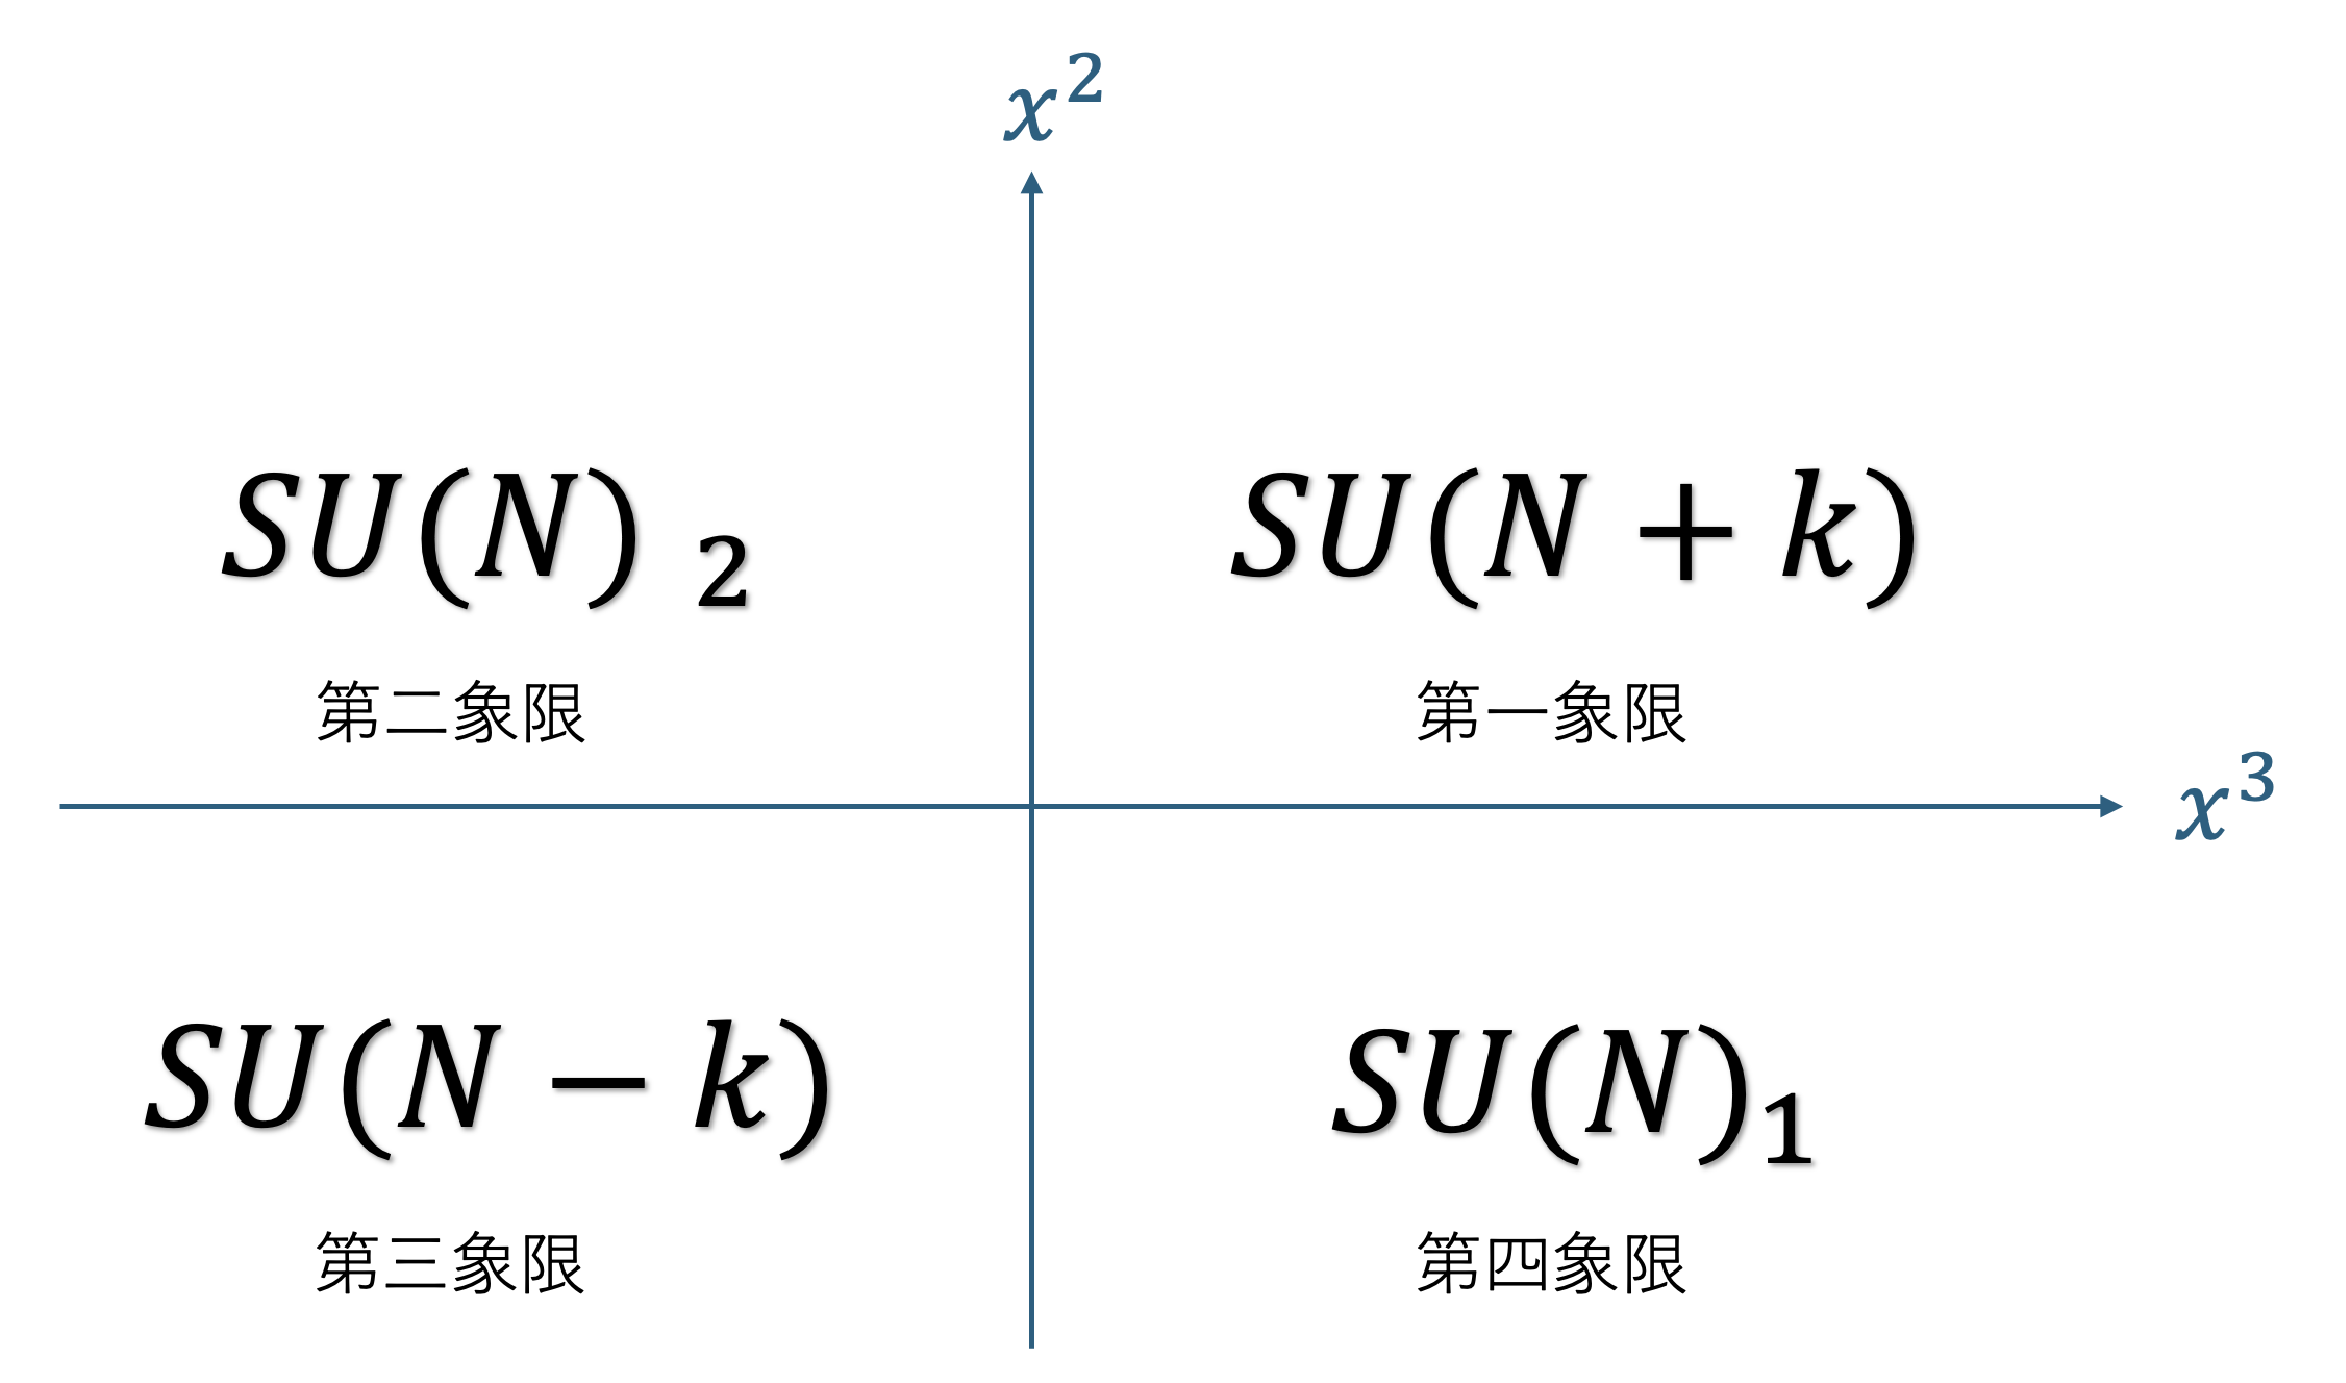
\includegraphics[scale=0.2]{Domain-wall-gauge.eps}
    \caption{Domain-wall}
    \label{fig:placeholder}
\end{figure}\\
この際、4つのリー代数の直和のリー代数やその部分群を構成するところから始めるのは非常に手間であるため、単一のDomain-wall系のFolding-trickから得られた帰結を元に、実用上となる特解を構成することに重きを置く。
\subsubsection{Domain-wall condition}
Diagonal部分群をゲージ群としてもつBoundary系からのDomain-wallを考えると、単一のDomain-wallの場合は、その帰結は以下の通りとなる。
\begin{resultbox}{diagonal部分群と双対なDomain-wall系}
    Domain-wall系は、共通のゲージを持つ部分が連続で、その直交補空間がD5-likeな境界条件となる。\\
    またこれは、$x^{3}=0$上だけでなく、$x^{2}=0$上でも同様の境界条件が成立する。
\end{resultbox}
\begin{proofbox}
    $x^{2}=0$周りの境界条件、モジュライ空間、Folding-trickを求める手続きは、$x^{3}=0$上での境界条件を求める手続きを、単に以下のように変更すれば得られるものである。
\begin{align*}
    \partial_{2}&\iff \partial_{3}\\
    A_{2}&\iff A_{3}\\
    B_{1}&\iff C_{2}\\
    X&\iff Y\\
\end{align*}
故に、$x^{3}=0$上と同様の論法が使える。
\end{proofbox}
CrossしたDomain-wall系を用いる場合は、各領域の境界に存在するDomain-wallに対してこれを行えばいい。\\
\\
まずは、embeddingによらない一般論を考える。Domain-wallは、以下のような4つが存在する。
\begin{enumerate}
        \item 1-2 Domain-wall($x^{2}\geq0,x^{3}=0$)
        \item 2-3 Domain-wall($x^{2}=0,x^{3}\leq0$)
        \item 3-4 Domain-wall($x^{2}\leq0,x^{3}=0$)
        \item 4-1 Domain-wall($x^{2}=0,x^{3}\geq0$)
\end{enumerate}
これらのDomain-wall間を行き来するためのembeddingとして、以下のようなものを定義する。
\begin{align*}
        &i_{41}:su(N)_{1}\to su(N+k)\\
        &i_{21}:su(N)_{2}\to su(N+k)\\
        &i_{34}:su(N-k)\to su(N)_{1}\\
    &i_{32}:su(N-k)\to su(N)_{2}
\end{align*}
このようなembeddingの下、各Domain-wallには以下のような境界条件が存在。ただし、embedding及びその部分群、直交補空間を表す添字のルールは、以下のように設定することにする。
\begin{defbox}{embeddingの添字のルール}
    第m象限から第n象限へのembedding、およびそれがなす部分空間、その直交補空間は、以下の添字の記法のもと表す。
    \begin{align*}
        i_{mn},h_{mn},h^{\perp}_{mn}
    \end{align*}
\end{defbox}
\begin{resultbox}{1-2 Domain-wall上($x^{2}\geq0,x^{3}=0$)の境界条件}
su(N+k)内に以下のような部分群が自然に存在。
    \begin{gather*}
        h_{21}=\{i_{21}(X)\in su(N+k)\,|\,X\in su(N)_{2}\}\\
        su(N+k)=h_{21}\oplus h_{21}^{\perp}
    \end{gather*}
    この場合、場は以下のように分解される。
    \begin{gather*}
        \Phi=\Phi^{h_{21}}+\Phi^{\perp_{21}}\\
        (\Phi^{h_{21}}\in h_{21},\quad \Phi^{\perp_{21}}\in h^{\perp_{21}})
    \end{gather*}
    そしてD5-like SUSYを保つDomain-wall上の境界条件は、以下のようになる。
    \begin{enumerate}
        \item $h_{21}$成分の境界条件
        \begin{align*}
            \Phi^{h_{21}}(x^{3}=+0)=\Phi(x^{3}=-0)
        \end{align*}
        \item 直交補空間上の境界条件
        \begin{gather*}
            (\varepsilon_{abc}D_{3}X_{a}^{\perp_{21}}-[X_{b}^{\perp_{21}},X_{c}^{\perp_{21}}]^{\perp_{21}})|_{x^{3}=+0,x^{2}\geq 0}=0\\
            Y^{\perp_{21}}|_{x^{3}=+0,x^{2}\geq 0}=0\\
            B_{1}\Psi^{\perp_{21}}|_{x^{3}=+0,x^{2}\geq 0}=\Psi^{\perp_{21}}
        \end{gather*}
    \end{enumerate}    
\end{resultbox}
\begin{resultbox}{2-3 Domain-wall上($x^{2}=0,x^{3}\leq0$)の境界条件}
    su(N)内に以下のような部分群が自然に存在。
    \begin{gather*}
        h_{32}=\{i_{32}(X)\in su(N)\,|\,X\in su(N-k)\}\\
        su(N)_{2}=h_{32}\oplus h_{32}^{\perp}
    \end{gather*}
    この場合、場は以下のように分解される。
    \begin{gather*}
        \Phi=\Phi^{h_{32}}+\Phi^{\perp_{32}}\\
        (\Phi^{h_{32}}\in h_{32},\quad \Phi^{\perp_{32}}\in h^{\perp_{32}})
    \end{gather*}
    そしてD5-like SUSYを保つDomain-wall上の境界条件は、以下のようになる。
    \begin{enumerate}
        \item $h_{32}$成分の境界条件
        \begin{align*}
            \Phi^{h_{32}}(x^{2}=+0)=\Phi(x^{2}=-0)
        \end{align*}
        \item 直交補空間上の境界条件
        \begin{gather*}
            X^{\perp_{32}}|_{x^{2}=+0,x^{3}\geq 0}=0\\
            (\varepsilon_{lmn}D_{2}Y_{l}^{\perp_{32}}-[Y_{m}^{\perp_{32}},Y_{n}^{\perp_{32}}]^{\perp_{32}})|_{x^{2}=+0,x^{3}\geq 0}=0\\
            C_{2}\Psi^{\perp_{32}}|_{x^{2}=+0,x^{3}\geq 0}=\Psi^{\perp_{32}}
        \end{gather*}
    \end{enumerate}    
\end{resultbox}
\begin{resultbox}{3-4 Domain-wall上($x^{2}\leq0,x^{3}=0$)の境界条件}
    su(N)内に以下のような部分群が自然に存在。
    \begin{gather*}
        h_{34}=\{i_{34}(X)\in su(N)\,|\,X\in su(N-k)\}\\
        su(N)_{1}=h_{34}\oplus h_{34}^{\perp}
    \end{gather*}
    この場合、場は以下のように分解される。
    \begin{gather*}
        \Phi=\Phi^{h_{34}}+\Phi^{\perp_{34}}\\
        (\Phi^{h_{34}}\in h_{34},\quad \Phi^{\perp_{34}}\in h^{\perp_{34}})
    \end{gather*}
    そしてD5-like SUSYを保つDomain-wall上の境界条件は、以下のようになる。
    \begin{enumerate}
        \item $h_{34}$成分の境界条件
        \begin{align*}
            \Phi^{h_{34}}(x^{3}=+0)=\Phi(x^{3}=-0)
        \end{align*}
        \item 直交補空間上の境界条件
        \begin{gather*}
            (\varepsilon_{abc}D_{3}X_{a}^{\perp_{34}}-[X_{b}^{\perp_{34}},X_{c}^{\perp_{34}}]^{\perp_{34}})|_{x^{3}=+0,x^{2}\leq 0}=0\\
            Y^{\perp_{34}}|_{x^{3}=+0,x^{2}\leq 0}=0\\
            B_{1}\Psi^{\perp_{34}}|_{x^{3}=+0,x^{2}\leq 0}=\Psi^{\perp_{34}}
        \end{gather*}
    \end{enumerate}    
\end{resultbox}
\begin{resultbox}{4-1 Domain-wall上($x^{2}=0,x^{3}\geq0$)の境界条件}
    まず、su(N+k)内に以下のような部分群が自然に存在。
    \begin{gather*}
        h_{41}=\{i_{41}(X)\in su(N+k)\,|\,X\in su(N)_{1}\}\\
        su(N+k)=h_{41}\oplus h_{41}^{\perp}
    \end{gather*}
    この場合、場は以下のように分解される。
    \begin{gather*}
        \Phi=\Phi^{h_{41}}+\Phi^{\perp_{41}}\\
        (\Phi^{h_{41}}\in h_{41},\quad \Phi^{\perp_{41}}\in h^{\perp_{41}})
    \end{gather*}
    そしてD5-like SUSYを保つDomain-wall上の境界条件は、以下のようになる。
    \begin{enumerate}
        \item $h_{41}$成分の境界条件
        \begin{align*}
            \Phi^{h_{41}}(x^{2}=+0)=\Phi(x^{2}=-0)
        \end{align*}
        \item 直交補空間上の境界条件
        \begin{gather*}
            X^{\perp_{41}}|_{x^{2}=+0,x^{3}\geq 0}=0\\
            (\varepsilon_{lmn}D_{2}Y_{l}^{\perp_{41}}-[Y_{m}^{\perp_{41}},Y_{n}^{\perp_{41}}]^{\perp_{41}})|_{x^{2}=+0,x^{3}\geq 0}=0\\
            C_{2}\Psi^{\perp_{41}}|_{x^{2}=+0,x^{3}\geq 0}=\Psi^{\perp_{41}}
        \end{gather*}
    \end{enumerate}    
\end{resultbox}
これが、embeddingの形を仮定しない一般的な場合のDomain-wall conditionである。\\
\\
今のようにDomain-wallが複数あ離、それが場合、十字状に伸びている場合、形から明らかなように、全てのDomain-wallが交わる交差点が存在する。以下では、このようなセットアップの際、Domain-wallの交差点がどのようになっているかを議論する。\\
\\
後々を考えると、$x^{2}=x^{3}=0$上で尚且つ、$h_{41}^{\perp}\cap h^{\perp}_{21}$上に存在するspinorのダイナミクスが非常に重要となる。このspinorには、例えば以下のような性質が存在する。
\begin{resultbox}{$x^{2}=x^{3}=0$上のspinorのchirality}
$h_{41}^{\perp}\cap h^{\perp}_{21}$上のspinorは、２次元の意味で、chiralityが正である。すなわち、
    \begin{align*}
        \Gamma_{0}\Gamma_{1}\Psi^{\perp}|_{cross}=\Psi^{\perp}
    \end{align*}
\end{resultbox}
\begin{proofbox}
    まず、10次元のChiral-spinorを用いているため、
    \begin{align*}
        \bar{\Gamma}\Psi^{\perp}=\Psi^{\perp}
    \end{align*}
    次に、境界条件より、
    \begin{align*}
        B_{1}\Psi^{\perp}|_{x^{3}=+0,x^{2}= +0}=\Psi^{\perp}\\
        C_{2}\Psi^{\perp}|_{x^{2}=+0,x^{3}= +0}=\Psi^{\perp}
    \end{align*}
    この３式と$B_{1},C_{2}$の定義より、上式が成立。
\end{proofbox}
ここまでが、embeddingの形を仮定しない、一般的な話である。\\

\subsubsection{embeddingの指定}
今、自分たちが行いたいのは一般論の構築でなく、あくまで特解の構築である。この特解を具体的に構築するためには、当然具体的なembeddingの情報が必要である。本小節ではembeddingを具体的に定義し、その図形的な記述法を与える。\\
ただし、本節以降、$k<N$を仮定する。\\
\\
本論では、以下のようなembeddingを採用することにする。
\begin{defbox}{$x^{2},x^{3}\geq 0$へのembedding}
    \begin{align*}
    &i_{41}(X)\equiv 
    \begin{pmatrix}
        X & 0_{N\times k}\\
        0_{k\times N} & 0_{k\times k}
    \end{pmatrix},\quad(X\in su(N)_{1})\\
    \\
    & i_{21}(X)\equiv 
    \begin{pmatrix}
        0_{k\times k} & 0_{k\times N}\\
        0_{N\times N} & X
    \end{pmatrix},\quad(X\in su(N)_{2})
\end{align*}
\end{defbox}
このようなembeddingを考えると、以下の性質が成立する。
\begin{resultbox}{embeddingの重なり}
    $i_{41}$,$i_{21}$の重なる部分の次元は、N-kである。
\end{resultbox}
\begin{proofbox}
    両者の重なる部分の次元をbとする。重ならない部分の次元を、両方aとする\footnote{両者対称であるため、重ならない部分の次元は一致する}。
    この時、次元勘定から以下のような連立方程式が成立する。
    \begin{align*}
        \begin{cases}
            a+b=N\\
            2a+b=N+k\\
        \end{cases}
    \end{align*}
    この方程式を解くと、$b=N-k$である。
\end{proofbox}
また、あと２つのembeddingとしては、以下のようなものを採用することにする。
    \begin{defbox}{$x^{2},x^{3}\leq 0$からのembedding}
    \begin{align*}
    &i_{34}(Y)\equiv 
    \begin{pmatrix}
        0_{k\times k} & 0_{ k\times (N-k)}\\
        0_{(N-k) \times k} & Y
    \end{pmatrix},\quad(Y\in su(N-k))\\
    \\
    & i_{32}(Y)\equiv 
    \begin{pmatrix}
        Y & 0_{(N-k)\times k }\\
        0_{k\times (N-k)} & 0_{k\times k}
    \end{pmatrix},\quad(Y\in su(N-k))
    \end{align*}
    \end{defbox}
$x^{2}=x^{3}=0$の交差点を考える際には、embeddingをさらにembeddingしたものを考えねばならない。embeddingの重なり部分の次元勘定から、su(N+k)内のこれらの次元の位置関係は、以下のように1枚の画像で表すことができる。
\begin{resultbox}{すべてのembeddingの位置関係}
    \begin{center}
  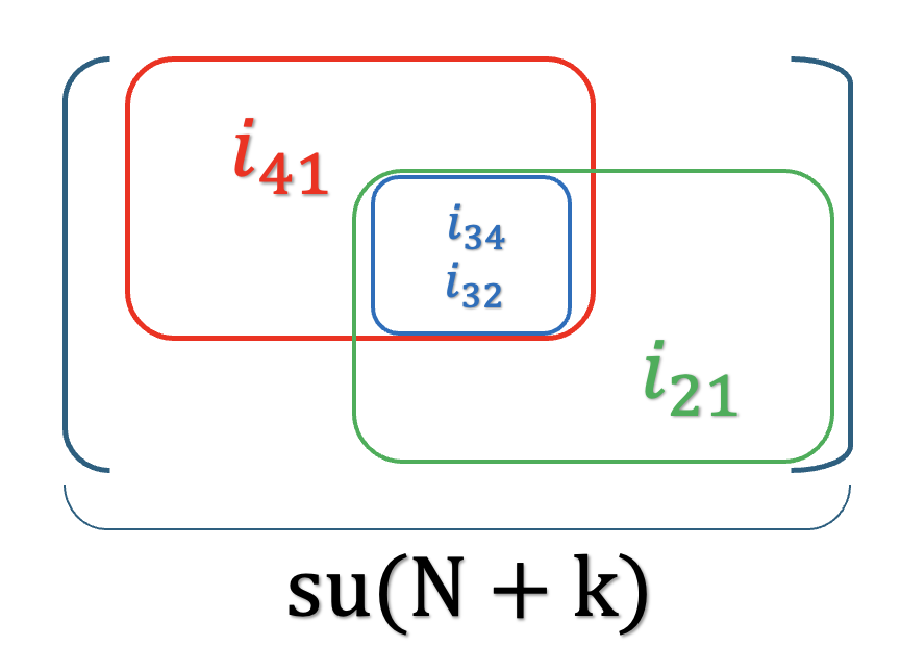
\includegraphics[width=0.5\linewidth]{embedding_domain-wall.eps}
  \captionof{figure}{埋め込み写像の位置関係}
\end{center}
\end{resultbox}
また、各embeddingの直交補空間がどのような位置関係になっているかも重要な情報である。それを図時すると、以下のようになる。
\begin{resultbox}{すべてのembeddingの位置関係}
    \begin{center}
  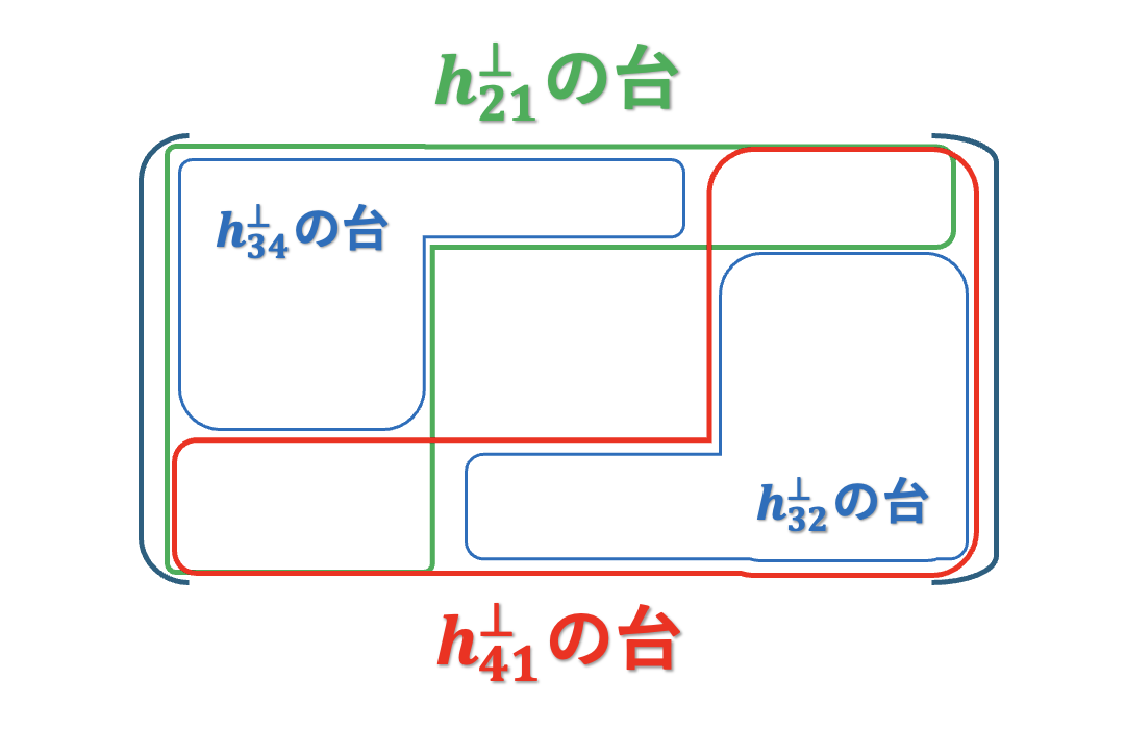
\includegraphics[width=0.5\linewidth]{perp_space.eps}
  \captionof{figure}{直交補空間の位置関係}
  ç
\end{center}
\end{resultbox}
これらのembeddingを考えると、$x^{2},x^{3}\leq0$のembeddingがなす部分空間、およびその直交補空間は、全て$x^{2},x^{3}\geq 0$の内部に包括されている。
\subsubsection{Vacuum expectation value}
以下では、このCrossしたDomain-wall系における、1/4-BPS分の超対称性を保つようなVEVの形について考察する。\\
まず、空間の対称性から。Boundaryの時に加えて、$D_{2}X_{a},D_{3}Y_{a},F_{01}$がそれぞれnon-zeroとなる。Boundaryの時のVEV-constraintの議論において、これらがnon-zeroであることを踏まえると、
\begin{resultbox}{Domain-wall系のBulk上のVEV}
        \begin{align*}
        0&=F_{01}\\
        0&=[X_{a},Y_{m}]\cdot\bar{\epsilon}_{0}B_{0}\\
    0&=\bar{\epsilon}_{0}([X_{b},X_{c}]-\epsilon_{abc}(D_{3}X_{a}B_{1}+D_{2}X_{a}C_{1}))\\
    0&=\bar{\epsilon}_{0}([Y_{m},Y_{n}]-\epsilon_{lmn}(D_{3}Y_{l}B_{2}+D_{2}Y_{m}C_{2}))\\
    \end{align*}
\end{resultbox}
これが、Bulkにおける1/4-BPSという条件からのVEVの制限である。
\subtopic{定数型のVEV}
Cross-Domain wall系のうち、まずはVEVの値が定数になるような状況を考える。\\
\\
この場合、まずはVEV-constraintの条件式は、以下のような形となる。
\begin{align*}
    &[X_{b},X_{c}]=[Y_{m},Y_{n}]=[X_{a},Y_{l}]=0
\end{align*}
故に、X,Yは全て同時対角化可能である。\\
\\
また、Domain-wall上の境界条件からVEVの値は制限を受ける。その結果どのようなVEVが許されるかを、各象限及びDomain-wallごとに考える。\\
\begin{enumerate}
    \item 第1象限($x^{2},x^{3}\geq0$)\\
    この象限における非自明な境界条件は、以下のようなものである。
    \begin{align*}
        &X_{a}^{\perp_{41}}|_{x^{2}=+0,x^{3}\geq 0}=0\\
        &Y_{m}^{\perp_{21}}|_{x^{2}\geq 0,x^{3}=+0}=0
    \end{align*}
    故に、第一象限におけるVEVの値は、以下の通りとなる。
    \begin{align*}
X=
\begin{pmatrix}
x_1 &        &        &        &  \\
    & \ddots &        &        &   \\
    &        & x_N    &        &   \\
    &        &        & 0      &   \\
   &        &        &        & 0
\end{pmatrix},
\qquad
Y=
\begin{pmatrix}
0   &        &        &        &  \\
    & \ddots &        &        &   \\
    &        & 0      &        &   \\
    &        &        & y_{N+1}&   \\
    &        &        &        & y_{N+k}
\end{pmatrix}.
    \end{align*}
    \item 第2象限($x^{2}\leq0,x^{3}\geq0$)\\
    第2象限上のVEVは、対角であることと定数であることから、以下のように表せる。
    \begin{align*}
        X=\begin{pmatrix}
\lambda_1 &        &          \\
    & \ddots &          \\
    &        & \lambda_N    
        \end{pmatrix}
        ,\quad
        Y=\begin{pmatrix}
\nu_1 &        &          \\
    & \ddots &          \\
    &        & \nu_N
        \end{pmatrix}
    \end{align*}
この時、1-2 Domain-wallにおける接続条件から、例えばX場のVEVについて、以下の関係が成立する。
\begin{align*}
    X(x^{3}\leq 0)=X^{h_{21}}(x^{3}\geq 0)
    \iff
    \begin{pmatrix}
        \lambda_1 &        &          \\
    & \ddots &          \\
    &        & \lambda_N  
    \end{pmatrix}
    =
    \begin{pmatrix}
x_{k+1} &        &        &        &  \\
    & \ddots &        &        &   \\
    &        & x_N    &        &   \\
    &        &        & 0      &   \\
   &        &        &        & 0
\end{pmatrix}
\end{align*}
この関係から、X場のVEVについては、以下の関係が成立する。
\begin{align*}
 X(x^{3}\leq 0)=\begin{pmatrix}
x_{k+1} &        &        &        &  \\
    & \ddots &        &        &   \\
    &        & x_N    &        &   \\
    &        &        & 0      &   \\
   &        &        &        & 0
\end{pmatrix}
\end{align*}
Y場も同様にして、以下のようなVEVの値が得られる。
\begin{align*}
    Y(x^{3}\leq 0)=\begin{pmatrix}
        y_1 &        &          \\
    & \ddots &          \\
    &        & y_N  
    \end{pmatrix}
\end{align*}
これが、1-2境界条件から縛られる、X,Y場のVEVの値である。\\
\\
また、2-3 Domain-wallの境界条件からの制限を考える。X,Y場に関する境界条件は以下の通りである。
\begin{align*}
    D_{2}Y^{\perp_{32}}|_{x^{2}=0}\\
    X^{\perp_{32}}|_{x^{2}=0}=0
\end{align*}
これらは、VEVの行列のexplicitな形を踏まえると、何ら新たな条件を出さないことがわかる。このため、VEVの値は、上で求めたものがそのまま成立する。\\
    \item 第4象限($x^{2}\geq0,x^{3}\leq0$)\\
    第2象限の時と同様の議論を行うと、以下のようなVEVの値が得られる。
    \begin{align*}
        X(x^{2}\leq 0)=\begin{pmatrix}
x_1 &        &          \\
    & \ddots &          \\
    &        & x_N    
        \end{pmatrix},\quad
        Y(x^{2}\leq 0)=\begin{pmatrix}
            y_{k+1} &        &        &        &  \\
    & \ddots &        &        &   \\
    &        & y_N    &        &   \\
    &        &        & 0      &   \\
   &        &        &        & 0
        \end{pmatrix}
    \end{align*}
    \item 第3象限($x^{2},x^{3}\leq0$)
    第2、第４象限からの接続条件の値から、以下のようなVEVの値が得られる。
    \begin{align*}
         X(x^{2},x^{3}\leq 0)=\begin{pmatrix}
        x_{k+1} &        &          \\
    & \ddots &          \\
    &        & x_N  
    \end{pmatrix}
    ,\quad
    Y(x^{2},x^{3}\leq 0)=\begin{pmatrix}
        y_{k+1} &        &          \\
    & \ddots &          \\
    &        & y_N  
    \end{pmatrix}
    \end{align*}
\end{enumerate}
以上の議論をまとめると、定数型のVEVの行列の形は、以下の１つのダイアグラムにまとめることが可能となる。
\begin{resultbox}{全空間における定数VEVの値}
    \begin{center}
  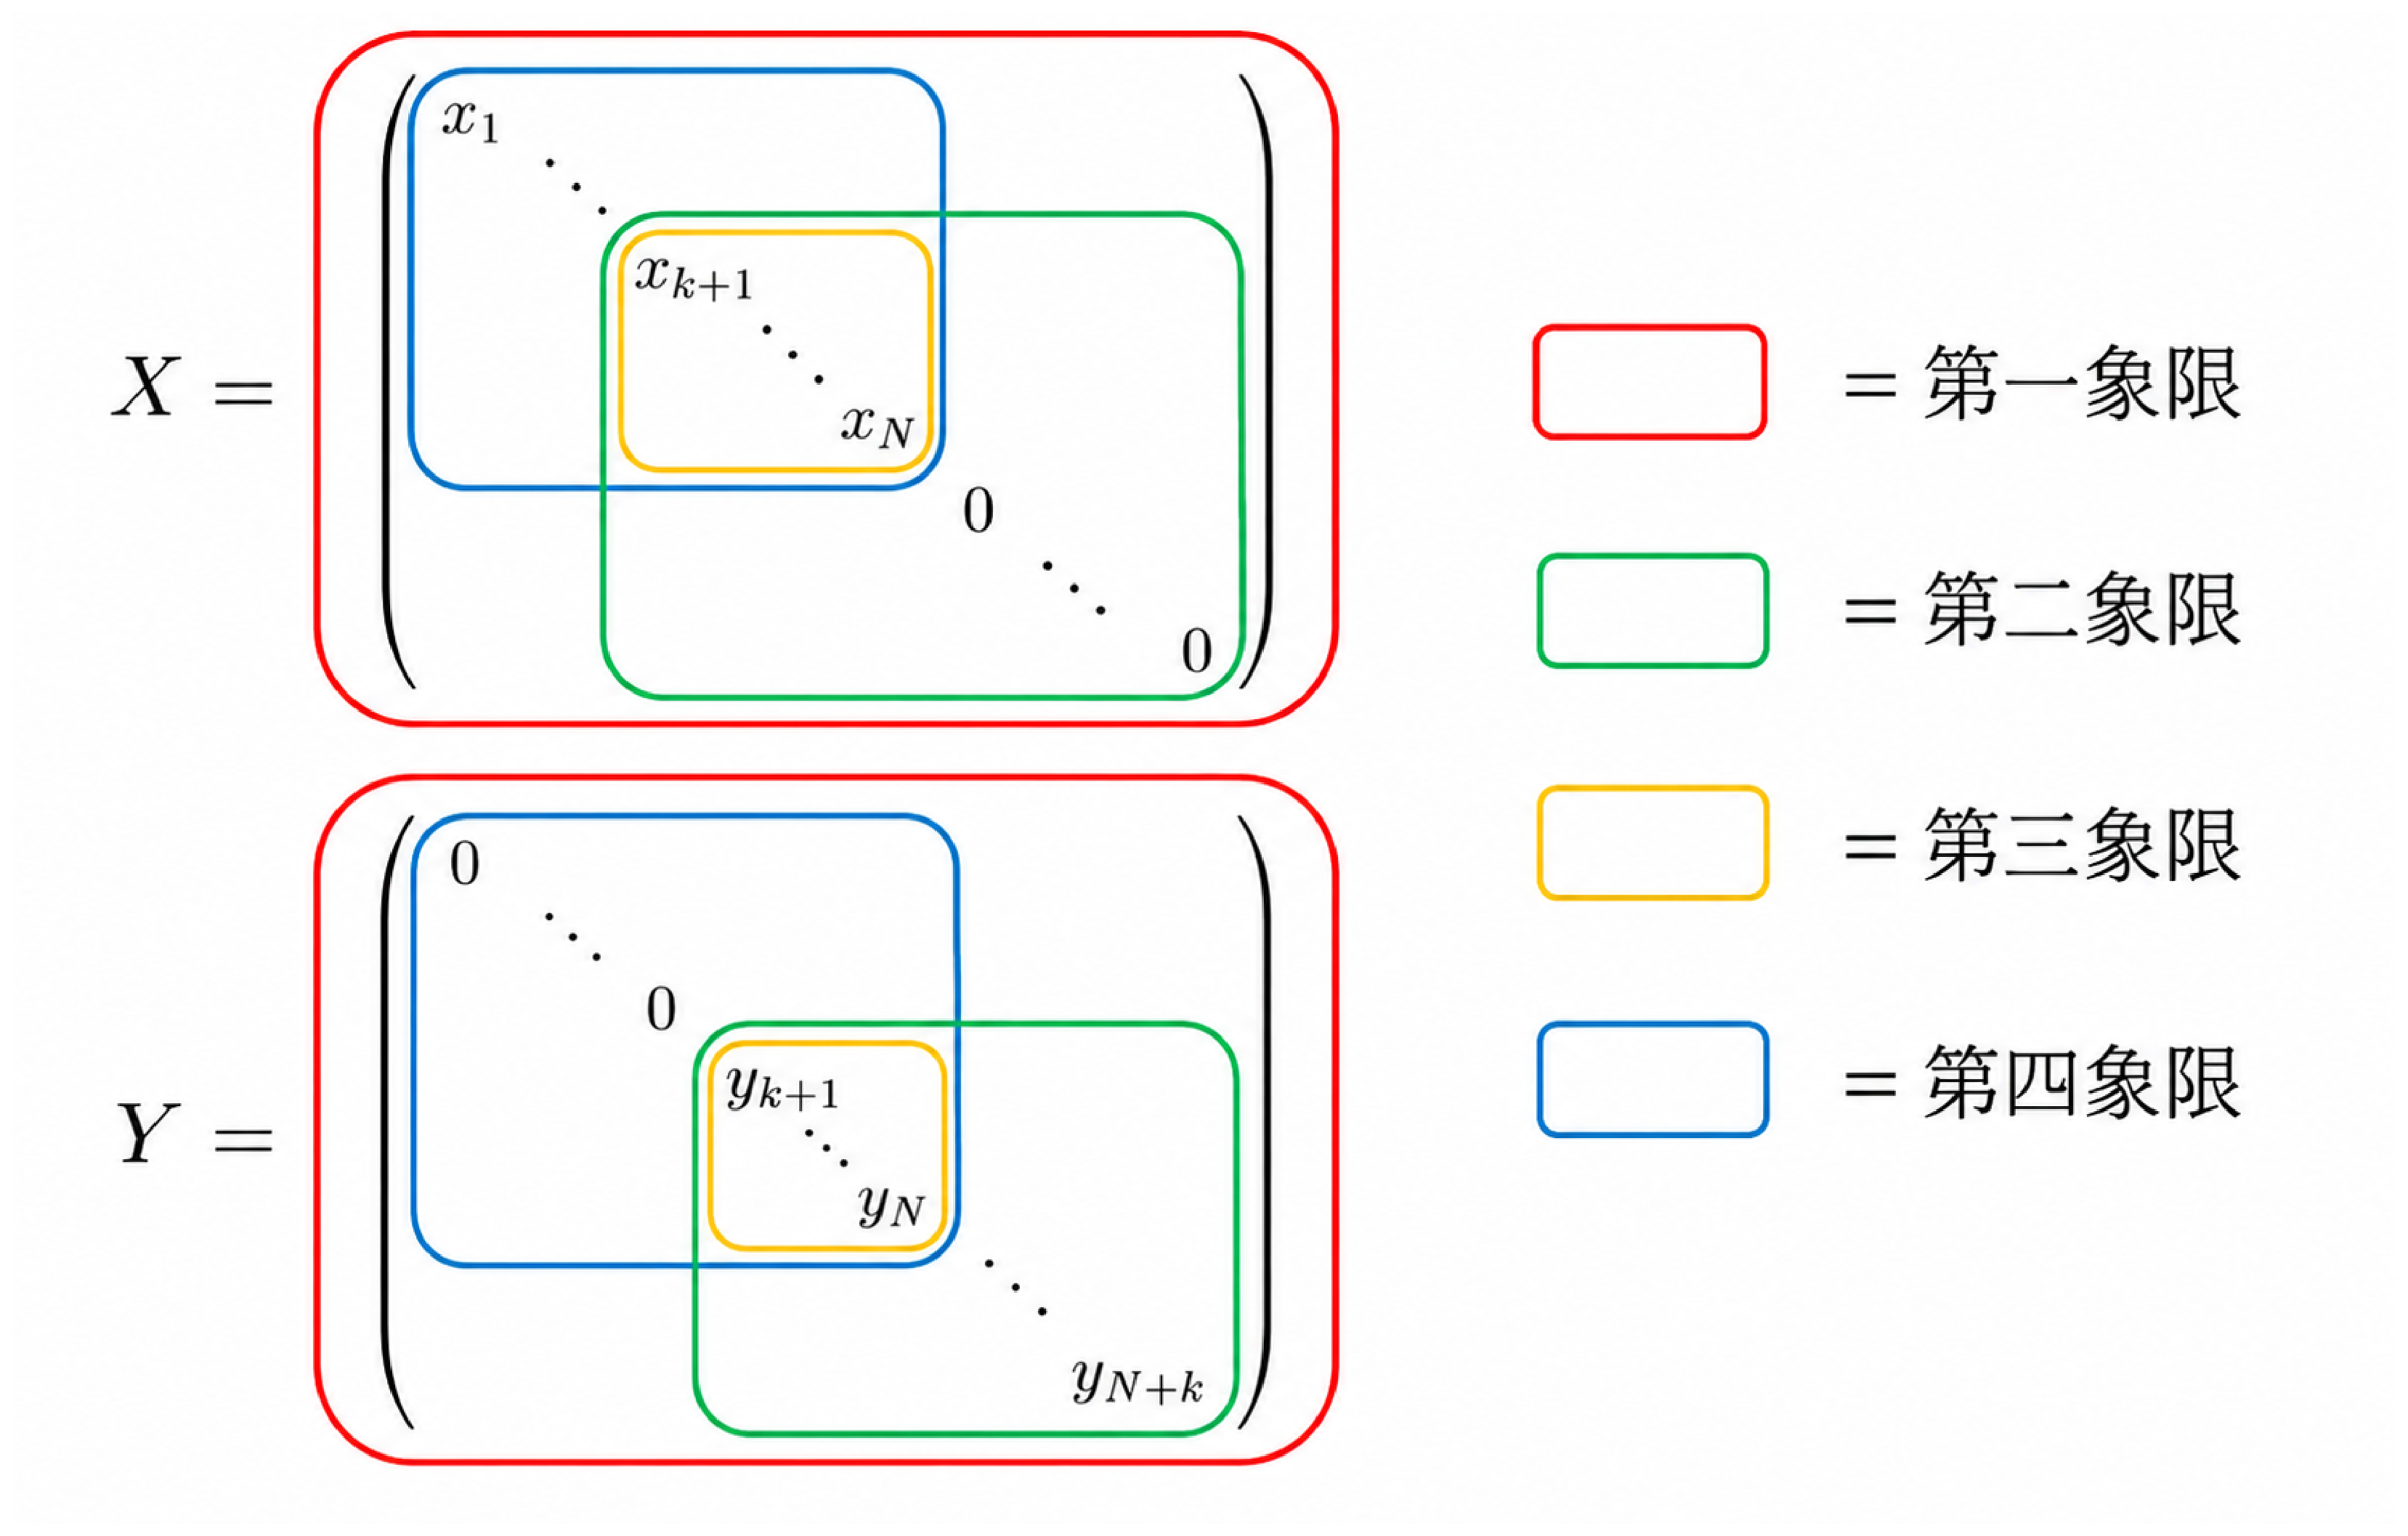
\includegraphics[width=0.5\linewidth]{VEV_area_crossing.eps}
  \captionof{figure}{全空間における定数VEVの値}
\end{center}
\end{resultbox}

\subtopic{Pole型のVEV}

\section{Localized Chiral zero mode}
Gauge-Anomalyはしばし、Weyl-fermionによって引き起こされる。特に、Anomaly-inflowの機構を考える場合、defect上に局在した、Weyl-fermionが非常に重要な役割を果たす。\\
ところで、一般に、D5-D5' Brane系においては、D5-D5'の交点に局在したWeyl-fermionにより、Anomaly-inflowが起こることが、stringの文脈において示されている。AdS/CFT対応の文脈から考えると、当然、双対となるd=4 N=4 SYM上でも同様に、Weyl-fermionがdefectの局在の上に存在し、Anomaly-inflowを再現するはずである。
以下、段階を追って、実際に、D3-D5-D5'系の、Domain-wall crossing系において、交点直上にWeyl-fermionが存在することを示す。

\subsection{Defect上のWeyl-fermionの一般論}
まずは、偶数次元に広がるdefect上にWeyl-fermionが存在することを示す際の、一般的な戦略について議論を行うことにする。\\
ただし、Hilbert空間全てで考えるとキリがないため、一旦、エネルギー固有値が一定の空間内でそのようなモードが実現する条件は何かを議論する。\\
\\
Weyl-fermionが存在することを示すためのセットアップは、以下の通りである。
\begin{setupbox}{Weyl-fermionの局在を示す手順}
    \begin{enumerate}
        \item 全体のDirac方程式、及び1粒子ハミルトニアンを書き下す
        \begin{gather*}
            i\Gamma^{\mu}\partial_{\mu}\Psi + (interaction-term)\Psi =0\\
            h=i\Gamma^{i}\partial_{i}+(interaction-term)
        \end{gather*}
        \item 1粒子ハミルトニアンを分ける\\
        1粒子ハミルトニアンを、defectが広がっている方向のkinetic-term $h_{int}$と、それ以外の部分$h_{ext}$に分解する。
        \begin{gather*}
            h=h_{int}+h_{ext}\\
            h_{int}=i\Gamma^{int}\partial_{int}\\
            h_{ext}=i\Gamma^{ext}\partial_{ext}+(interaction)
        \end{gather*}
        ただし、この時${h_{int},h_{ext}}=0$かを確かめる。成立しないなら、この方法は使えないので、引き上げる。
        \item defect上のChirality行列$\bar{\gamma_{int}}$と$h_{ext}$が反可換かを調べる
        \begin{enumerate}
            \item 反可換でない場合\\
            この方法は使えないので、引き上げる。
            \item 反可換であった場合
            以下の方程式の、normalizedな解を探す。
            \begin{align*}
                h_{ext}\Psi=0
            \end{align*}
            解が存在するならば、その解がlocalized Weyl-fermionである。
        \end{enumerate}
    \end{enumerate}
\end{setupbox}
以下、上記のセットアップで得られた解が、確かにlocalized Weyl-fermionであることを示す。正確なstatementは以下の通りである。
\begin{resultbox}{defect上のWeylの存在条件}
    以下の条件を仮定する。
    \begin{gather*}
        \{h_{int},h_{ext}\}=0\\
        \{h_{ext},\bar{\gamma}_{int}\}=0\\
    \end{gather*}
    この時、$\Psi$がdefect上にWeyl-fermionが局在するモードである必要十分条件は、以下の通りである。
    \begin{align*}
         h_{ext}\Psi =0
    \end{align*}
\end{resultbox}
\begin{proofbox}
    まず、hの固有モードと$h_{ext}$の固有モードの対応を関連づけるため、$h^{2}$を考える。この時、$\{h_{int},h_{ext}\}=0$であるため、
    \begin{gather*}
        h^{2}=h^{2}_{int}+h^{2}_{ext}
    \end{gather*}
    ここで、仮定$\{h_{int},h_{ext}\}=0$より、
    \begin{align*}
        [h^{2}_{int},h_{ext}^{2}]=[h^{2},h_{int}^{2}]=[h^{2},h_{ext}^{2}]=0
    \end{align*}
    故に$h^{2}_{int},h_{ext}^{2}$は同時対角化可能。また、defectに沿う方向には並進対称性が残っているため、その固有関数はフーリエモードであることが自明である。故に、h,ひいては$h^{2}$のモードを扱うことは、$h_{ext}^{2}$のモードを扱うことに等しい。
\end{proofbox}
\subsection{Boundary上に局在したlocalized Weyl-mode}

\subsection{D3-D5-D5' system上のlocalized Weyl-mode}

\appendix
\section{Shurの補題}
このセクションでは、Pole解を構成、分類するときに非常に重要となる、Shurの補題について解説する。まずはShurの補題のAssumptionを述べるために、以下の概念を導入する。

\begin{defbox}{g準同型}
群gの２つの表現$(\rho_{V},V),(\rho_{W},W)$が存在したとする。この2つの表現が「g準同型」であるというのは、以下の関係を満たす$f_{0}:V\to W$が存在することを意味する。
\begin{align*}
    f_{0}\rho_{V}(X)=\rho_{W}(X)f_{0}
\end{align*}
また、2つの表現が「g同型」であるというのは、「2つの表現がg準同型かつ、その時のfが全単射である」ことを意味する。
\end{defbox}
この時、shurの補題のstatementは以下である。
\begin{theorembox}{shurの補題1}
群gの２つの「既約」表現$(\rho_{V},V),(\rho_{W},W)$が存在し、以下の関係を満たす$f:V\to W$が存在したとする。
\begin{align*}
    f\rho_{V}(X)=\rho_{W}(X)f
\end{align*}
この時、以下のstatementが成立する。
\begin{enumerate}
    \item 2つの表現がg準同型でない$\implies f=0$ 
    \item 2つの表現がg準同型$\implies f=\lambda f_{0}$ 
\end{enumerate}
\end{theorembox}
また、ここから直ちに導かれる結果として、以下が挙げられる。これもshurの補題と呼ばれている。
\begin{theorembox}{shurの補題2}
群gの既約表現を$(\rho_{V},V)$とする。
\begin{align*}
    f\rho_{V}(X)=\rho_{V}(X)f \implies f=\lambda I_{dimV}
\end{align*}
\end{theorembox}
以下では、shurの補題の証明ではなく、「使い方」として、導かれる帰結をいくつか紹介する。特に、2番目の結果は、Pole解を構成、分類する際に大きな役割を果たす。
\begin{resultbox}{Abelianの既約表現}
    Abel群の既約表現は1次元である。
\end{resultbox}
\begin{proofbox}
    Abel群の表現として、($\rho_{V},V$)が存在したとする。これは定義より、以下の関係式を満たす。
    \begin{align*}
        \rho_{V}(g_{1})\rho_{V}(g_{2})=\rho_{V}(g_{2})\rho_{V}(g_{1})
    \end{align*}
    この時、$\rho_{V}(g_{2})=f$とおくと、shurの補題２から、以下が言える。
    \begin{align*}
        f=\rho_{V}(g_{2})=\lambda I_{dimV}
    \end{align*}
    この時、$dimV\neq 1$なら、既約性に反するため、$dimV=1$となる。故に、Abel群の既約表現は、必ず１次元表現になる。
\end{proofbox}
次の性質の証明に行く前に、SU(2)の表現において重要な性質をいくつか述べる。
\begin{resultbox}{SU(2)表現の性質}
    \begin{enumerate}
    \item (SU(2)に限らず)ユニタリ表現は完全可約である。
    \item SU(2)のN次元既約表現は1種類しか存在しない。
    \end{enumerate}
\end{resultbox}
\begin{proofbox}
    \begin{enumerate}
        \item ユニタリ表現の完全可約性\\
        これを示すためには、以下のlemmaを示せれば良い。
        \begin{theorembox}{lemma}
        ($\rho_{V},V$)を群の表現とする。また、Vの不変部分空間をW、Wの直交補空間を$W^{\perp}$とする。
        \begin{align*}
            \text{($\rho_{V},V$)がユニタリ表現}\implies \text{$W^{\perp}$も不変部分空間}
        \end{align*}
        \end{theorembox}
        \begin{proofbox}
            このlemmaは以下と同値である。
            \begin{align*}
                \vec{w}\in W^{\perp}\implies \rho_{V}(X)\vec{w}\in W^{\perp}
            \end{align*}
            故にこれを示れば良い。ユニタリ表現を考えているため、定義から表現空間上に内積$<,>$が存在している。この時、$\vec{v}\in W,\vec{w}\in W^{\perp}$とすると、以下が成立する。
            \begin{align*}
                <\vec{v},\rho(X)\vec{w}>=<\rho(X)^{\dagger}\vec{v},\vec{w}>=<\rho(X)\vec{v},\vec{w}>=0
            \end{align*}
            ただし、第２式への変形は、ユニタリ内積の定義を用いて、第３式への変形は、表現がユニタリであることの条件を用いた。\\
            このため、$\vec{w}\in W^{\perp}\implies \rho_{V}(X)\vec{w}\in W^{\perp}$は示された。
        \end{proofbox}
        このlemmaの下、可約なユニタリ表現は順次直和に分解される。これをすべての表現が既約になるまで繰り返すことができるため、ユニタリ表現は完全可約である。
        \item SU(2)既約表現の一意性\\
        すまんが全部書くのは流石にしんどい。リー代数のノートを見てくれ。
    \end{enumerate}
\end{proofbox}
上記のSU(2)の表現の性質と、shurの補題を用いると、以下の結果を導くことができる。これが、Pole解の分類を行う際に非常に重要な指針となる。
\begin{resultbox}{N次元SU(2)表現の性質}
\begin{enumerate}
    \item SU(2)のN次元表現は、既約分解で何次元表現が出てくるかで、一意に指定される。そのため、SU(2)N次元表現は、以下で記述される。
    \begin{align*}
        N=\sum_{i}N_{i}
    \end{align*}
    ただし、右辺の数字は既約表現の次元である。
    \item SU(N)内でのSU(2)N次元表現との可換な部分がなすリー代数pは、N次元表現内の$N_{i}$表現の数を$M_{i}$とすると、以下のように記述できる。
    \begin{align*}
        p=SU(M_{1})\times SU(M_{2})\cdots
    \end{align*}
\end{enumerate}
\end{resultbox}
\begin{proofbox}
\begin{enumerate}
    \item SU(2)N次元表現の指定方法\\
    SU(2)表現の性質から、直ちに従う。
    \item SU(2)と可換な部分リー代数pについて\\
    一般論の証明を初手から行うのは難しいので、いくつかのケースで、この主張が成立することを、まずは確認する。
    \begin{enumerate}
        \item 3=1+2次元表現の場合\\
        この時、SU(2)の3次元表現は以下のように記述可能である。
        \begin{align*}
            \rho(T^{a})=
            \begin{pmatrix}
           \frac{1}{2}\sigma^{a} & 0 \\0 & 0
            \end{pmatrix}
        \end{align*}
        これに対して、SU(3)の基本表現を、一般に以下のように記述する。
        \begin{align*}
            s=\begin{pmatrix}
           V_{2\to 2} & V_{2\to1} \\V_{1\to 2} & V_{1\to 1}
            \end{pmatrix}
        \end{align*}
        以下、sのうち、上記の$\rho(T^{a})$と可換な部分は何かについて考える。sと$\rho(T^{a})$の交換関係は以下のように記述される。
        \begin{align*}
            [s,\rho(T^{a})]=\begin{pmatrix}
           [\frac{1}{2}\sigma^{a},V_{2\to 2}] & \frac{1}{2}\sigma^{a}V_{1\to 2} \\ \frac{1}{2}V_{2\to 1}\sigma^{a}& 0
            \end{pmatrix}
        \end{align*}
        可換であるためには、当然交換関係は0でなければならない。パウリ行列が逆行列を持つことを加味すると、そのためには、以下が要請される。
        \begin{align*}
            \frac{1}{2}\sigma^{a}V_{1\to 2}=0&\implies V_{1\to 2}=0\\
            \frac{1}{2}V_{2\to 1}\sigma^{a}=0&\implies V_{2\to1}=0\\
            [\frac{1}{2}\sigma^{a},V_{2\to 2}]=0&\implies \sigma^{a}V_{2\to 2}=V_{2\to 2}\sigma^{a}\\
            &\implies V_{2\to2 }=\lambda I_{2\times 2}
        \end{align*}
        故に、su(2)3=2+1表現と可換な部分リー代数pは、以下の通りとなる。
        \begin{align*}
            p=<\begin{pmatrix}
           I_{2} & 0 \\ 0& 0
            \end{pmatrix}> \approx U(1)\\
        \end{align*}

        \item 4=2+2表現の場合\\
        この場合、su(2)表現は以下のように記述される。ただし、$\sigma'$はパウリ行列の別基底である。
         \begin{align*}
            \rho(T^{a})=
            \begin{pmatrix}
           \frac{1}{2}\sigma^{a} & 0 \\0 & \frac{1}{2}\sigma'^{a}
            \end{pmatrix}
        \end{align*}
        この時、SU(4)の成分を以下のように記述する。
       \begin{align*}
            s=\begin{pmatrix}
           V_{2\to 2} & V_{2\to2'} \\V_{2'\to 2} & V_{2'\to 2'}
            \end{pmatrix}
        \end{align*}
        sと$\rho(T^{a})$の交換関係は、以下の通りである。
        \begin{align*}
            [s,\rho(T^{a})]=\begin{pmatrix}
           [\frac{1}{2}\sigma^{a},V_{2\to 2}] & \frac{1}{2}\sigma^{a}V_{2'\to 2}-\frac{1}{2}V_{2'\to 2}\sigma'^{a} \\ \frac{1}{2}\sigma^{a}V_{2\to 2'}-\frac{1}{2}V_{2\to 2'}\sigma'^{a}& [\frac{1}{2}\sigma^{a},V_{2'\to 2'}]
            \end{pmatrix}=0
        \end{align*}
    各成分に対してshorの補題を適用すると、以下の対応が言える。ただし、ここでは簡単のため、$\sigma'^{a}=\sigma^{a}$とする。一般論は別基底であるため、非対角成分のIがg準同型写像fとなる。
    \begin{align*}
        s=\begin{pmatrix}
            aI_{2}&bI_{2}\\
            cI_{2}&dI_{2}
        \end{pmatrix}=\begin{pmatrix}
            a&b\\
            c&d
        \end{pmatrix}\otimes I_{2}\equiv A\otimes I_{2}
    \end{align*}
    尚且つ、sはSU(4)の元であるという要請から、以下が言える。
    \begin{align*}
        Tr A=0,\quad A^{\dagger}+A=0
    \end{align*}
    以上を踏まえると、4=2+2成分と可換な部分群は、以下の通りとなる。
    \begin{align*}
        p=<A\otimes I_{2}>\approx su(2)
    \end{align*}
    \item 4=2+1+1の時\\
    上記と似たような式変形を辿ると、4=2+1+1と可換な部分群は、以下の通りとなる
    \begin{align*}
        p=su(2)\oplus u(1)
    \end{align*}
    \end{enumerate}
これらの例を一般化すると、表題となる。
    
\end{enumerate}
\end{proofbox}
\section{リー代数の内積}
この章では、リー代数の内積の構造についてまとめる。まず、いくつかの数学の言葉を定義する。
\begin{defbox}{リー代数のイデアル}
    リー代数のイデアルとは、以下を満たすリー代数の部分集合である。
    \begin{align*}
        \text{(イデアル)}=\{X\in g \,|\forall Y\in g,[X,Y]\in \text{(イデアル)}\,\}
    \end{align*}
\end{defbox}
\begin{defbox}{単純、半単純}
リー代数が半単純であるとは、可換なイデアルを持たないことをいう。
リー代数が単純であるとは、イデアルを持たないことをいう。
\end{defbox}
ここで、リー代数の不変内積の自然なメトリックとして、以下のようなメトリックを定義できる。
\begin{defbox}{リー代数内積のメトリック}
$T^{i}$・・・リー代数の生成子\\
$ad(X)$・・・リー代数XのAdjoint表現\\
\begin{align*}
    g_{ij}\equiv Tr(Ad(T_{i})Ad(T_{j}))
\end{align*}
\end{defbox}
重要な性質として、以下が挙げられる。
\begin{resultbox}{半単純リー代数のメトリック}
\begin{align*}
    \text{リー代数が半単純}\iff detg\neq 0
\end{align*}
\end{resultbox}
この定理は、非退化内積(すべてのベクトルとの内積が0になるベクトルが、ゼロベクトルしかないような内積)を持つリー代数が、半単純or単純しかあり得ないことを指している。\\
\\
例えば、このメトリックの他にも、リー代数の基本表現の内積を考えるようなメトリックも存在する。この場合、一般的に以下のような関係が成立する。
\begin{resultbox}{リー代数の内積}
    \begin{align*}
        <X,Y>\propto tr_{Ad}(Ad(X)Ad(Y))
    \end{align*}
\end{resultbox}
故に、基本表現に基づく内積の定義も、Adjointに基づく内積の精々定数倍しか違わない。故に、内積をAdjointにしたところで、なんの不都合も生じない。\\

\end{document}
